%% Anchor — CS 160 Summer 2026 final paper (team Hi-Five Senses)
%% Cleaned-up version of sigplan.tex. Compile with pdfLaTeX (Overleaf: default).
\documentclass[sigplan,screen]{acmart}

%% Class project: no ACM copyright block or reference strip.
\setcopyright{none}
\settopmatter{printacmref=false}
\renewcommand\footnotetextcopyrightpermission[1]{}
\acmConference[CS 160 '26]{COMPSCI 160: User Interface Design and Development}{Summer 2026}{UC Berkeley}
\acmYear{2026}
\usepackage{float}

\begin{document}

\title{Anchor: Steady the Day}

\author{Sampurn Bhowmick}
\email{sampurn.bhowmick@berkeley.edu}
\affiliation{%
  \institution{University of California, Berkeley}
  \city{Berkeley}
  \state{California}
  \country{USA}}

\author{Na Mi Kim}
\email{nami\_kim0401@berkeley.edu}
\affiliation{%
  \institution{University of California, Berkeley}
  \city{Berkeley}
  \state{California}
  \country{USA}}

\author{Madison Bryna Lee}
\email{madison.bryna@berkeley.edu}
\affiliation{%
  \institution{University of California, Berkeley}
  \city{Berkeley}
  \state{California}
  \country{USA}}

\author{Thanhbinh Nguyen}
\email{thanhbinh@berkeley.edu}
\affiliation{%
  \institution{University of California, Berkeley}
  \city{Berkeley}
  \state{California}
  \country{USA}}

\author{Reed Yalouh}
\email{yalouh@berkeley.edu}
\affiliation{%
  \institution{University of California, Berkeley}
  \city{Berkeley}
  \state{California}
  \country{USA}}

\renewcommand{\shortauthors}{Bhowmick et al.}

\begin{abstract}
Students and young adults managing mental health challenges such as ADHD, anxiety, and depression often struggle not with planning or organization, but with initiation due to a sense of overwhelm from having too much to do: the moment of beginning an already-understood task. Through needfinding interviews with seven participants, we found that existing productivity tools have not addressed the core issues, which are lack of initiation and fear of overwhelm.

We designed and built Anchor, a mobile-first web application that consolidates scattered obligations from Google Calendar and Gmail into a single, bounded daily plan of three tasks, each paired with a small, concrete first step. Anchor closes the loop from a morning briefing through a focus timer to an evening reflection, with unfinished work automatically carried forward rather than lost.

We iterated in low- and high-fidelity prototypes, incorporating feedback from 12 participants in paper and Figma prototype testing, before implementing a functional version using React, Supabase, and the Google Calendar and Gmail APIs. This document documents our full design process from needfinding through evaluation and outlines our planned next iteration.
\end{abstract}

\begin{CCSXML}
<ccs2012>
 <concept>
  <concept_id>10003120.10003121.10003122.10003331</concept_id>
  <concept_desc>Human-centered computing~Usability testing</concept_desc>
  <concept_significance>500</concept_significance>
 </concept>
 <concept>
  <concept_id>10003120.10003121.10003122.10003334</concept_id>
  <concept_desc>Human-centered computing~User studies</concept_desc>
  <concept_significance>500</concept_significance>
 </concept>
</ccs2012>
\end{CCSXML}

\ccsdesc[500]{Human-centered computing~Usability testing}
\ccsdesc[500]{Human-centered computing~User studies}

\keywords{task initiation, procrastination, ADHD, anxiety, depression, morning briefing, focus timer, reflection}

%% ------------------------------------------------------------------
%% Optional teaser figure (full-width image between authors and body).
%% To use it: put your image (e.g. teaser.png) in this folder, then
%% uncomment the block below.
%%
%% \begin{teaserfigure}
%%   \includegraphics[width=\textwidth]{teaser}
%%   \caption{Anchor's daily loop: morning briefing, three anchors, focus session, evening reflection.}
%%   \Description{Four app screenshots side by side showing the main screens of Anchor.}
%%   \label{fig:teaser}
%% \end{teaserfigure}
%% ------------------------------------------------------------------

\maketitle

\noindent\textbf{Project Website:} \url{https://sane24.github.io/Anchor-Design-Journal/}

\section{Introduction}
For many students and young professionals who experience challenges such as ADHD, anxiety, or depression, the hardest part of completing tasks is often not the work itself, but figuring out where to start. Our needfinding revealed two interconnected barriers: overwhelm from having too much to do and difficulty initiating tasks. One participant had every prerequisite for a task ready for a year—number found, script written, insurance card saved—but still could not start because the task had no clear starting or ending point. Another had no trouble finishing tasks once he started working, but the mental effort and preparation required often caused him to delay until the last minute. Across participants, scattered obligations across emails, calendars, and chats, combined with ambiguous task requirements, made it difficult to determine what to prioritize or do first, increasing feelings of anxiety and overwhelm.

This paper introduces Anchor, an application designed to reduce this cognitive overload and make starting feel more manageable. Rather than asking users to organize an endless list of responsibilities themselves, Anchor pulls scattered obligations into one place and operates on a simple, grounded philosophy: steady the day by limiting daily focus to three core tasks, or what we call “Anchors.” By narrowing an overwhelming set of responsibilities into a small number of priorities and identifying a concrete first step for each, Anchor aims to reduce cognitive overload, break through initiation paralysis, and turn stressful, chaotic work sessions into calmer, more intentional progress.

Anchor was developed by a five-person team, Hi-Five Senses, over six weeks in UC Berkeley’s COMPSCI 160 summer course. Across needfinding, lo-fi and hi-fi prototyping, implementation, and user evaluation, we repeatedly returned to the same core challenge: how to help people overcome the overwhelm that makes starting a task so difficult.

\section{Needfinding}
We are redesigning the experience of starting and completing work for people with mental health challenges such as ADHD, anxiety, or depression. Our focus is on how people regulate focus, motivation, and emotions through virtual systems, physical spaces, and personal routines, and how these supports can be improved to reduce overwhelm and make progress feel more achievable.

\subsection{Participants and POV Statements}
We recruited non-CS 160 students and recent graduates with ADHD, anxiety, depression, or similar mental health challenges. These participants were chosen because they regularly navigate demanding work and school responsibilities while managing their mental health, which makes them representative of the users we hope to support. We finished observation and interview sessions: a high school student with a busy schedule, a fourth-year math major student with ADHD and depression, a recent graduate and new software engineer with self-diagnosed anxiety, a recent electrical engineering graduate with anxiety, a senior with OCD and ADHD in a dual-degree program, a fourth-year environmental economics student juggling coursework, research, and an internship; and a senior balancing two remote jobs and a class.

\subsection{Methods}
During each session, we observed how participants began working on a real work or study task in their natural environment. Some participants allowed us to observe and take notes on their home workspace. We then conducted semi-structured interviews about their productivity habits, challenges with starting and completing tasks, sources of stress, and strategies and tools they use to stay organized. We paid particular attention to workarounds, breakdowns, current methods, and why those methods failed.

\subsection{Findings}
A pattern emerged as we synthesized point-of-view statements across the seven sessions: the gap was difficulty starting, not planning. Although participants often had detailed plans and full task lists, they still became stalled at initiation. We also found that organization alone did not increase motivation. Several findings stood out:
\begin{enumerate}
  \item Downscoping works. When an overwhelming call was reduced to ``only need to find the phone number and insurance information,'' participants could finish preparing in 5 minutes without distraction. Low-threshold tasks can be initiated easily, but unbounded tasks cannot.
  \item Tasks without edges are hard to begin. Open-ended tasks with no clear starting points easily sat undone for months or years even with every prerequisite ready.
  \item Entry point matters. One participant mentioned that she needs a start in a familiar location with coffee, and fully-charged devices.
  \item Ambiguity amplifies stress. Unstructured tasks are the most mentioned factor that causes a sense of overwhelm, and fear.
  \item Self-report feels fake. One participant tried the gamified habit app Habitica and abandoned it because self-checking boxes decrease motivation instead of increasing it.
  \item People create urgency and fallbacks. Participants created fake deadlines (``I will call at three'') and regard their social circle as a motivational engine.
\end{enumerate}

From these sessions, we synthesized thirteen "How Might We" questions spanning distraction reduction, task breakdown, cognitive overload, and social accountability. Two questions have proved most generative for our eventual design direction: how might we lower the barrier to starting unscheduled, open-ended tasks with no clear start or end, and how might we help students reduce the cognitive overload that precedes procrastination in the first place.

\section{Design Space and Concept Selection}
Each team member independently selected two rough ideas that they wanted to explore further. Using divergent brainstorming techniques, we expanded each concept into 2--3 distinct variations. Our brainstorming explored different interaction modalities, including web and mobile applications, browser extensions, wearable smart glasses, AR/VR, and physical interfaces.

\subsection{Funneling to Three Realizations}
We funneled these distinct ideas into 3 candidate realizations, drew concept sketches, and explicitly listed pros and cons:
\begin{enumerate}
  \item Users can select the apps which are  distracting to them. The app button and interfaces of the rest of the apps remain colorful, but the longer the users stay on the distraction apps, the grayer the interfaces and the app buttons become.

  \begin{figure}[!htbp]
    \centering
    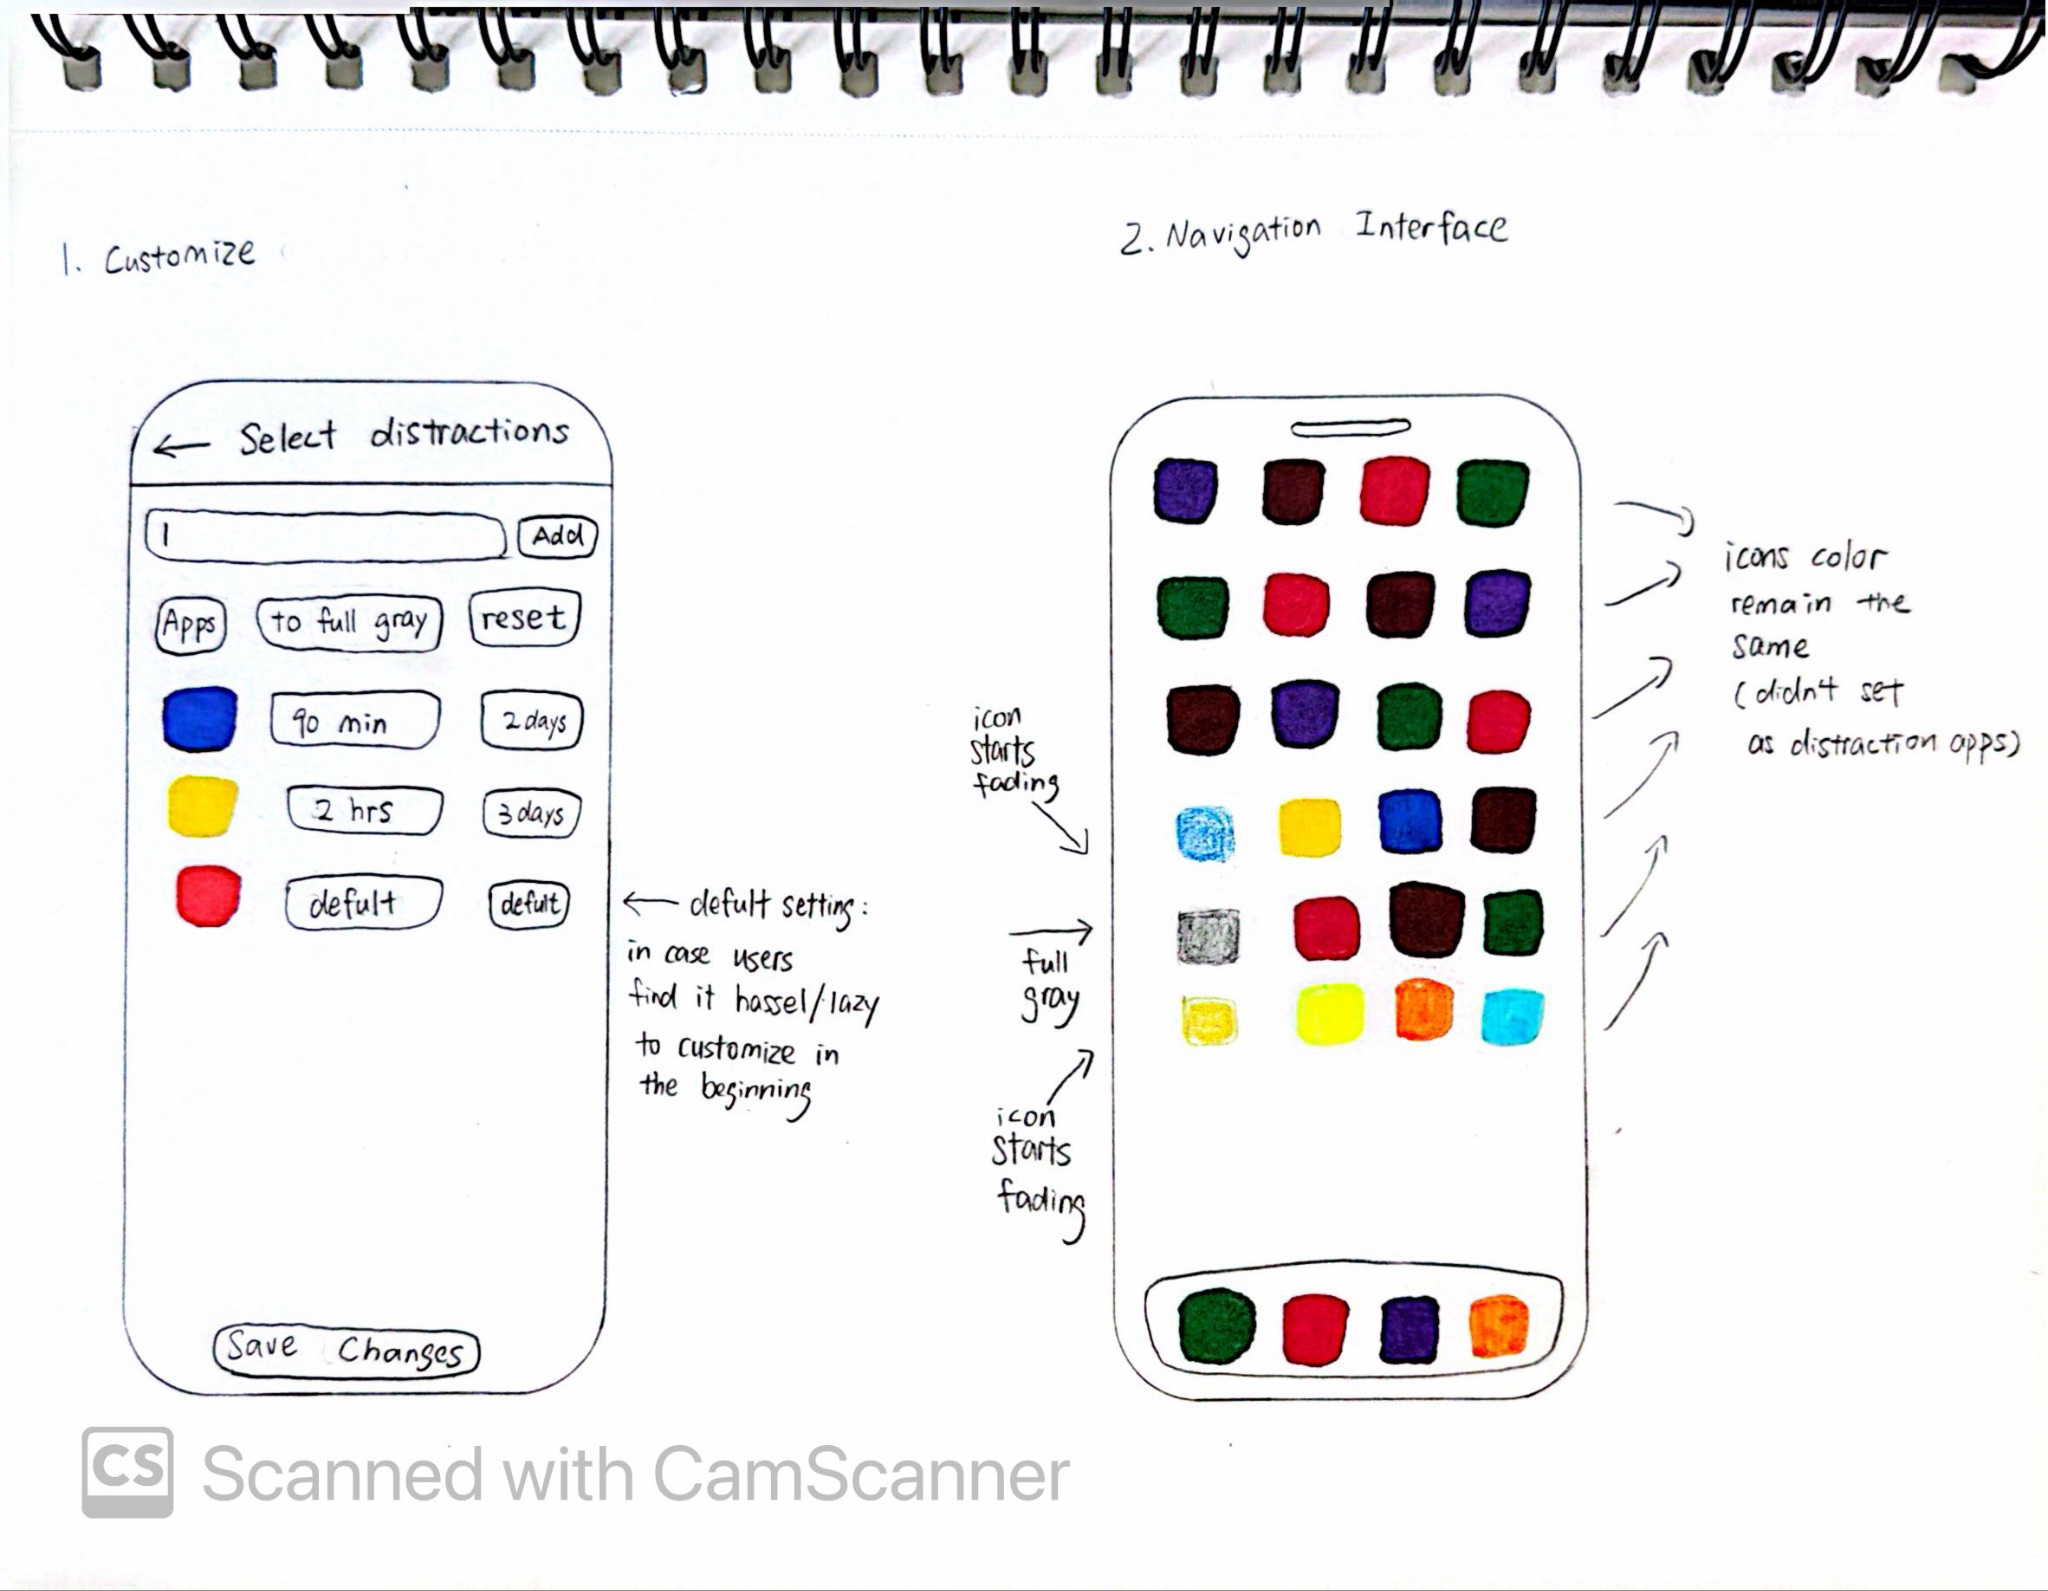
\includegraphics[width=.95\linewidth]{sketch-grayscale-ui.png}\\[4pt]
    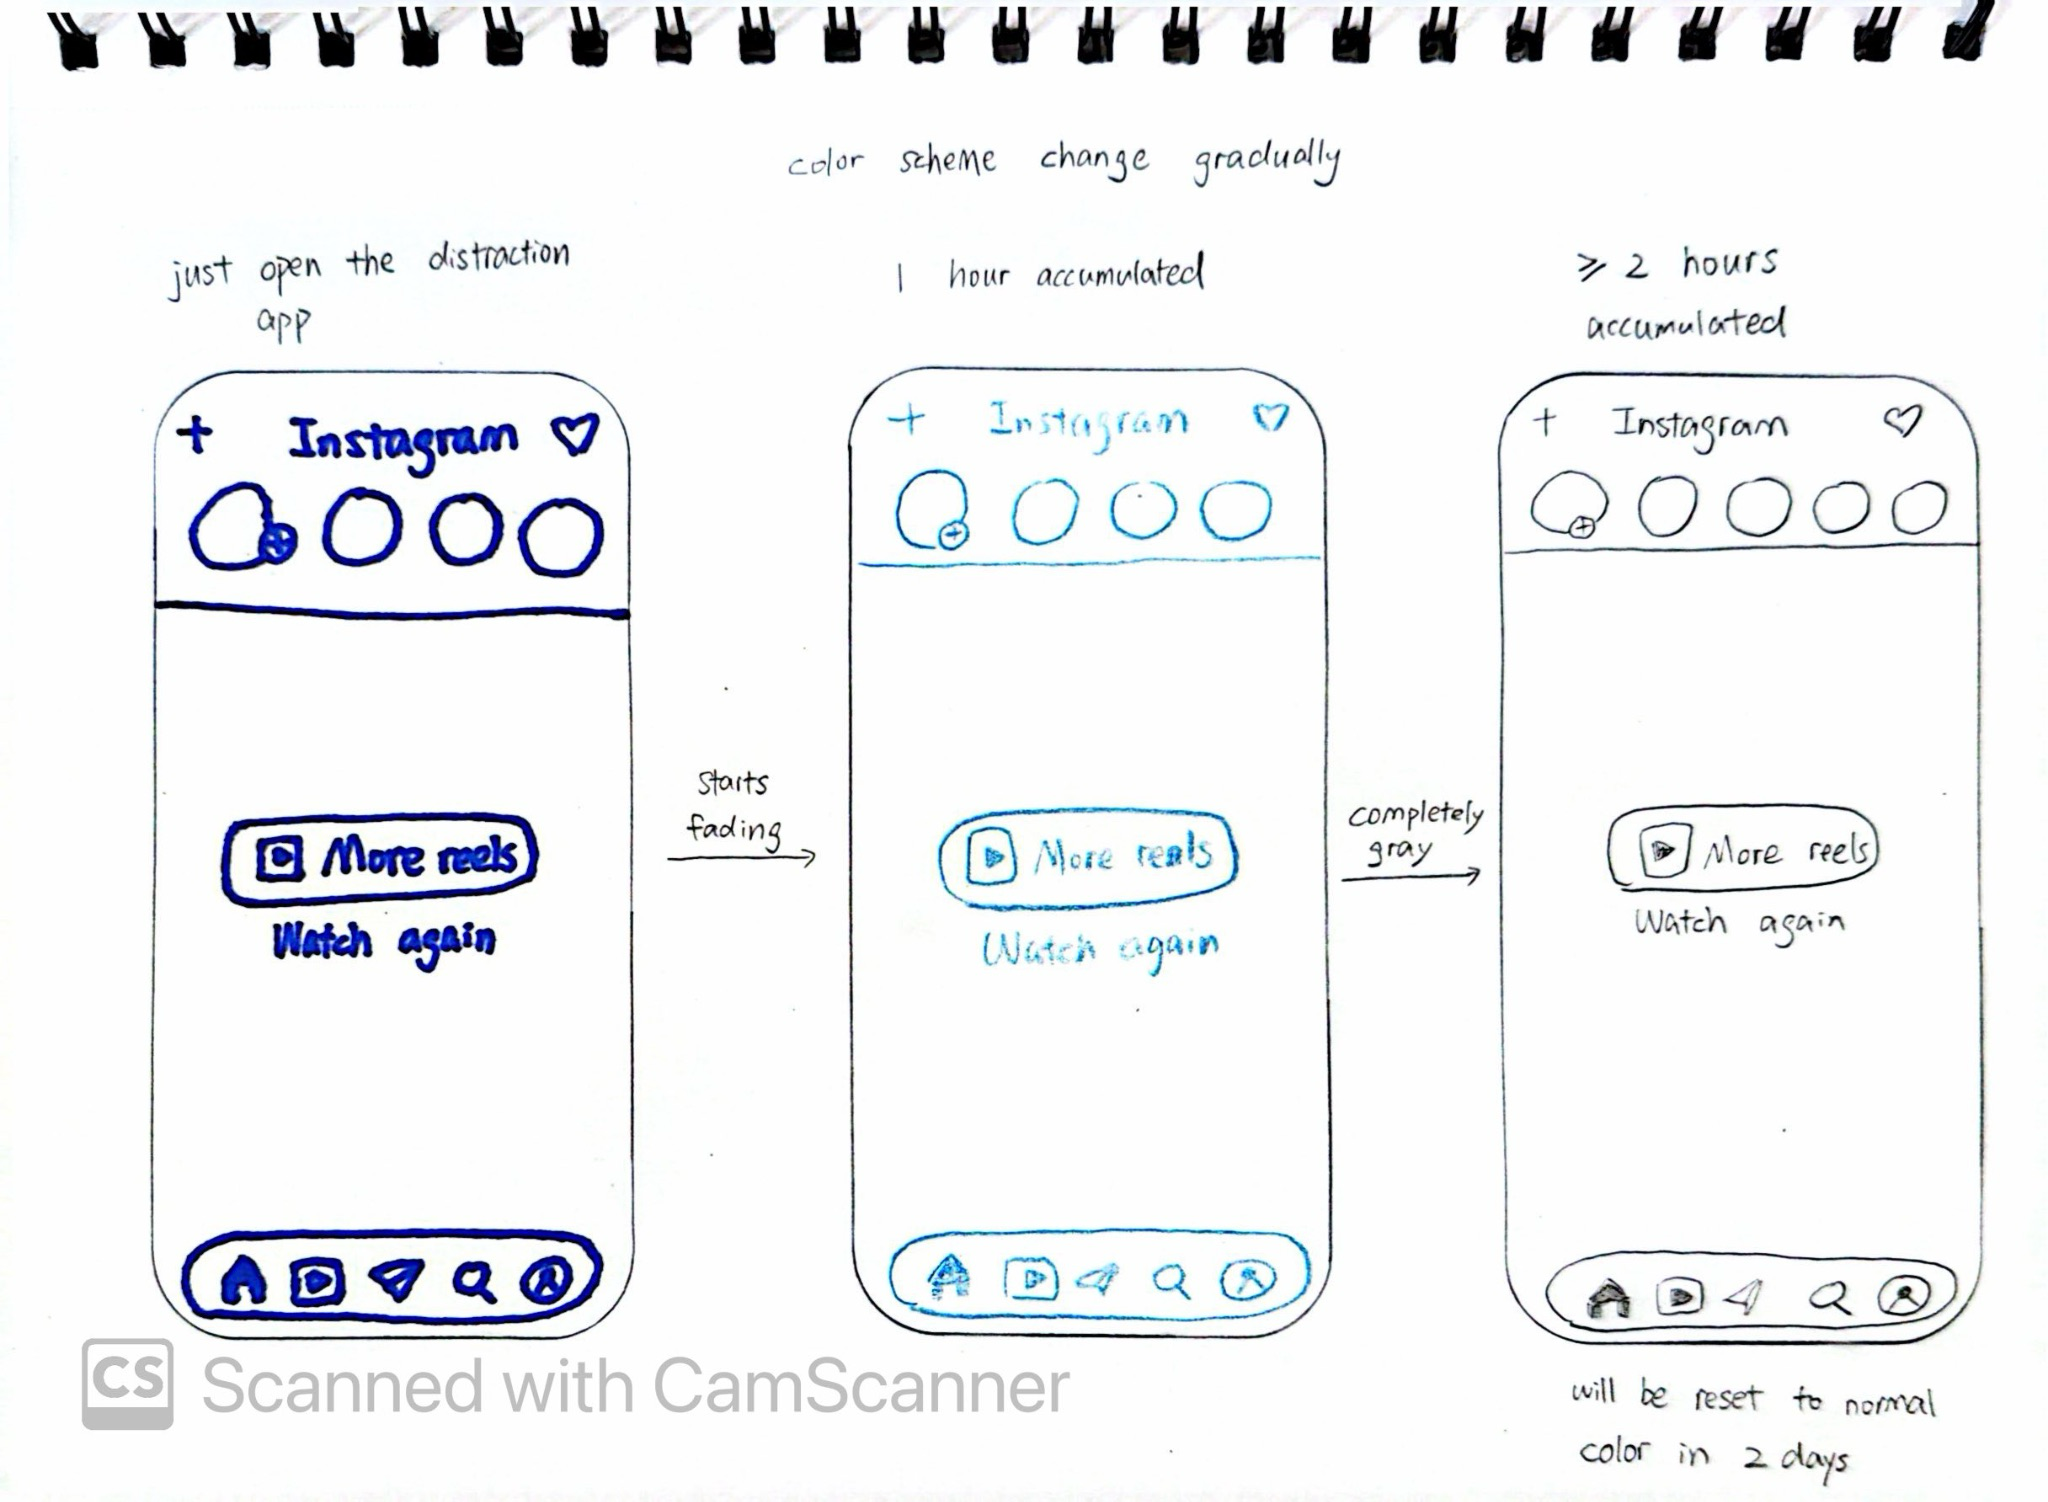
\includegraphics[width=.95\linewidth]{sketch-grayscale-fading.png}
    \caption{Concept sketches for realization 1: selecting distracting apps and gradually fading their interfaces to grayscale.}
    \Description{Two hand-drawn mobile interface sketches showing distraction-app selection and an app progressively losing color during continued use.}
    \label{fig:funnel-grayscale}
  \end{figure}

  \item Unified weekly, morning, and night briefings that turn scattered responsibilities into a bounded daily plan.

  \begin{figure}[!htbp]
    \centering
    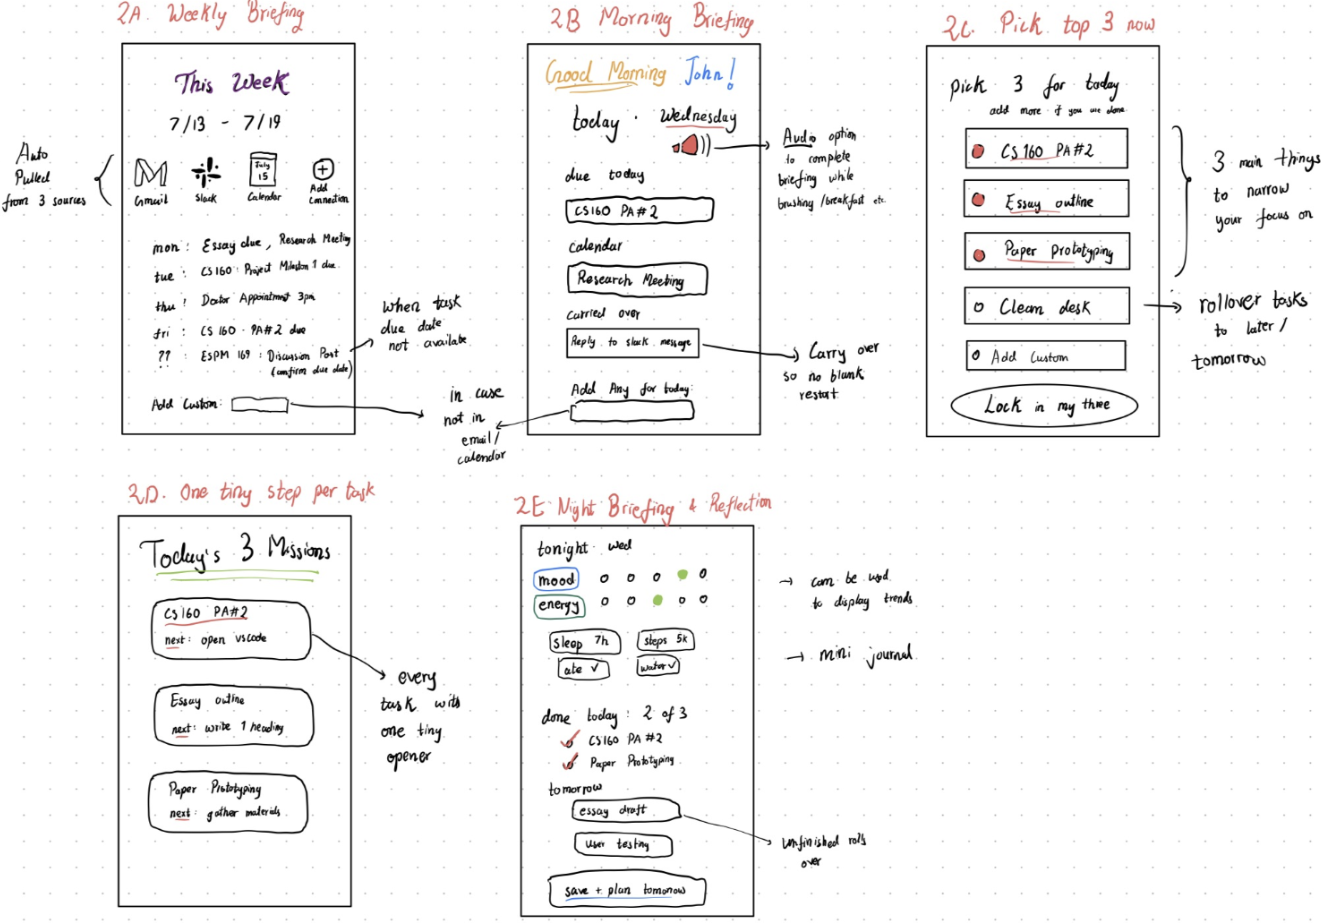
\includegraphics[width=.95\linewidth]{sketch-briefing.png}
    \caption{Concept sketch for realization 2: unified weekly, morning, and night briefings.}
    \Description{Hand-drawn mobile screens for a weekly briefing, morning briefing, Pick 3, daily mission board, and night briefing and reflection.}
    \label{fig:funnel-briefing}
  \end{figure}

  \item An accountability companions application, that allows users to set both personal and shared goals with their friends, track task progress, send encouragement, maintain shared streaks, and stay accountable. Through an optional AR mode, users can also study alongside a friend or accountability buddy in a shared virtual workspace, creating a stronger sense of co-presence while working.

  \begin{figure}[!htbp]
    \centering
    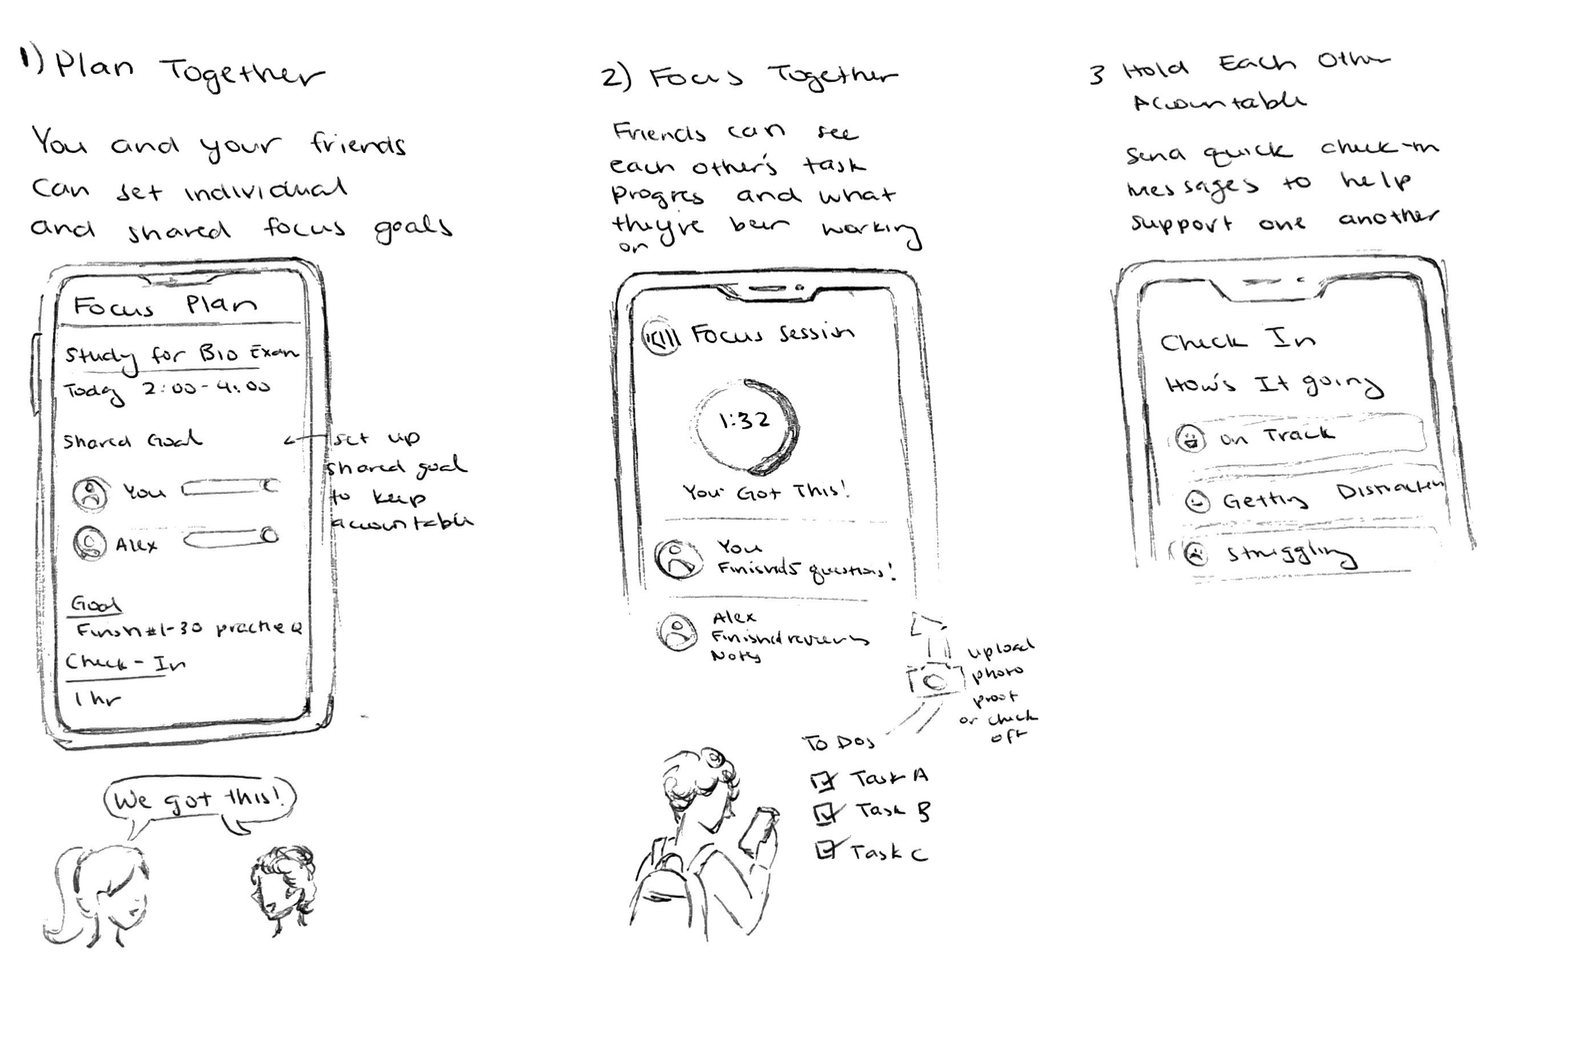
\includegraphics[width=.95\linewidth]{sketch-buddy-flow1.png}\\[4pt]
    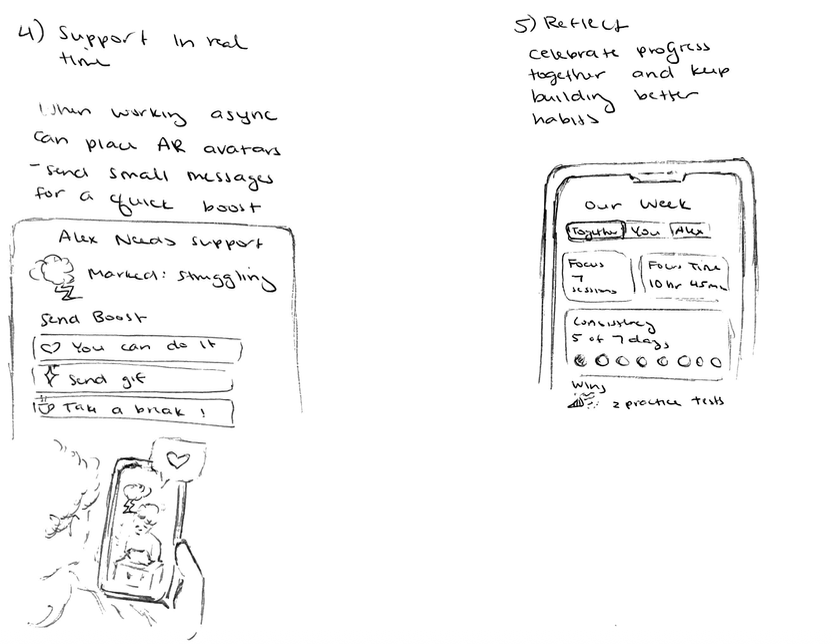
\includegraphics[width=.95\linewidth]{sketch-buddy-flow2.png}
    \caption{Concept sketches for realization 3: planning, focusing, mutual support, and weekly reflection with an accountability companion.}
    \Description{Two hand-drawn concept sheets showing friends creating shared goals, focusing together, checking in, supporting each other, and reviewing weekly progress.}
    \label{fig:funnel-buddy}
  \end{figure}
\end{enumerate}
\subsection{Final Selection: Unified Briefings}
We chose Unified Briefings because the idea targets the actual barrier our interviews surfaced, which is initiation and cognitive overload, not information or planning. One participant had every prerequisite ready for a year (number found, script written, insurance card saved) and still couldn't begin because the task had no bounded start or end. By pulling scattered obligations from Gmail, Slack, and Calendar into one plan and narrowing each day to a single tiny next action, this design gives open-ended tasks the edges that make starting possible, meets people in tools they already use, and closes the loop from morning to night with rollover so no one opens a blank page. This also prevents the analysis paralysis of having too many things to do so you don't know where to start. The other two realizations solve narrower problems: grayscale apps address distraction, but our participant was clear that ``it's not just distraction, it's that you don't want to do it,'' and the buddy system leans on social accountability, which risks the shame and rejection sensitivity that make ADHD and anxiety users abandon systems in the first place.

\section{Lo-fi Prototyping}
We made two paper prototypes with the same basic functionality but varying interfaces based on the idea we selected, expecting users to accomplish 3 defined tasks:
\begin{enumerate}
  \item Plan today from scattered inputs. Start briefing and gather tasks from Gmail/Slack/Calendar. Goal: go from ``something's due somewhere at some time'' to a locked top 3 for today, each with a first step. Success: 3 missions chosen, each showing one tiny next step.
  \item Start the next action. Goal: find and begin the single smallest next step for the priority task, without having to decide what to do. Success: user starts the opener.
  \item Close out the day and roll over. Goal: log a quick mood, energy, and care check, mark what got done, carry unfinished work forward. Success: reflection saved, unfinished tasks appear in tomorrow's plan.
\end{enumerate}

Each prototype was tested with 3 users with the think-aloud method.

\subsection{Two Paradigms}
\textbf{Prototype A: Stepped briefing and dashboard} with structured screens, one decision per screen (Figure~\ref{fig:protoa}). A mobile app with one main full-screen view per stage of the day. Each screen is a dense, scannable surface: the weekly briefing shows source tags (mail, slack, calendar) above a day-grouped list of obligations, the morning briefing groups today's items into due, calendar, and carried-over sections, pick-top-3 is a selectable list, today's missions shows the three chosen tasks each with a tiny next step, and night reflection combines mood and energy dot-scales, care anchors, a done count, and a tomorrow list. Everything on a screen is visible at once, and the user reads and taps directly.

\begin{figure}[!ht]
  \centering
  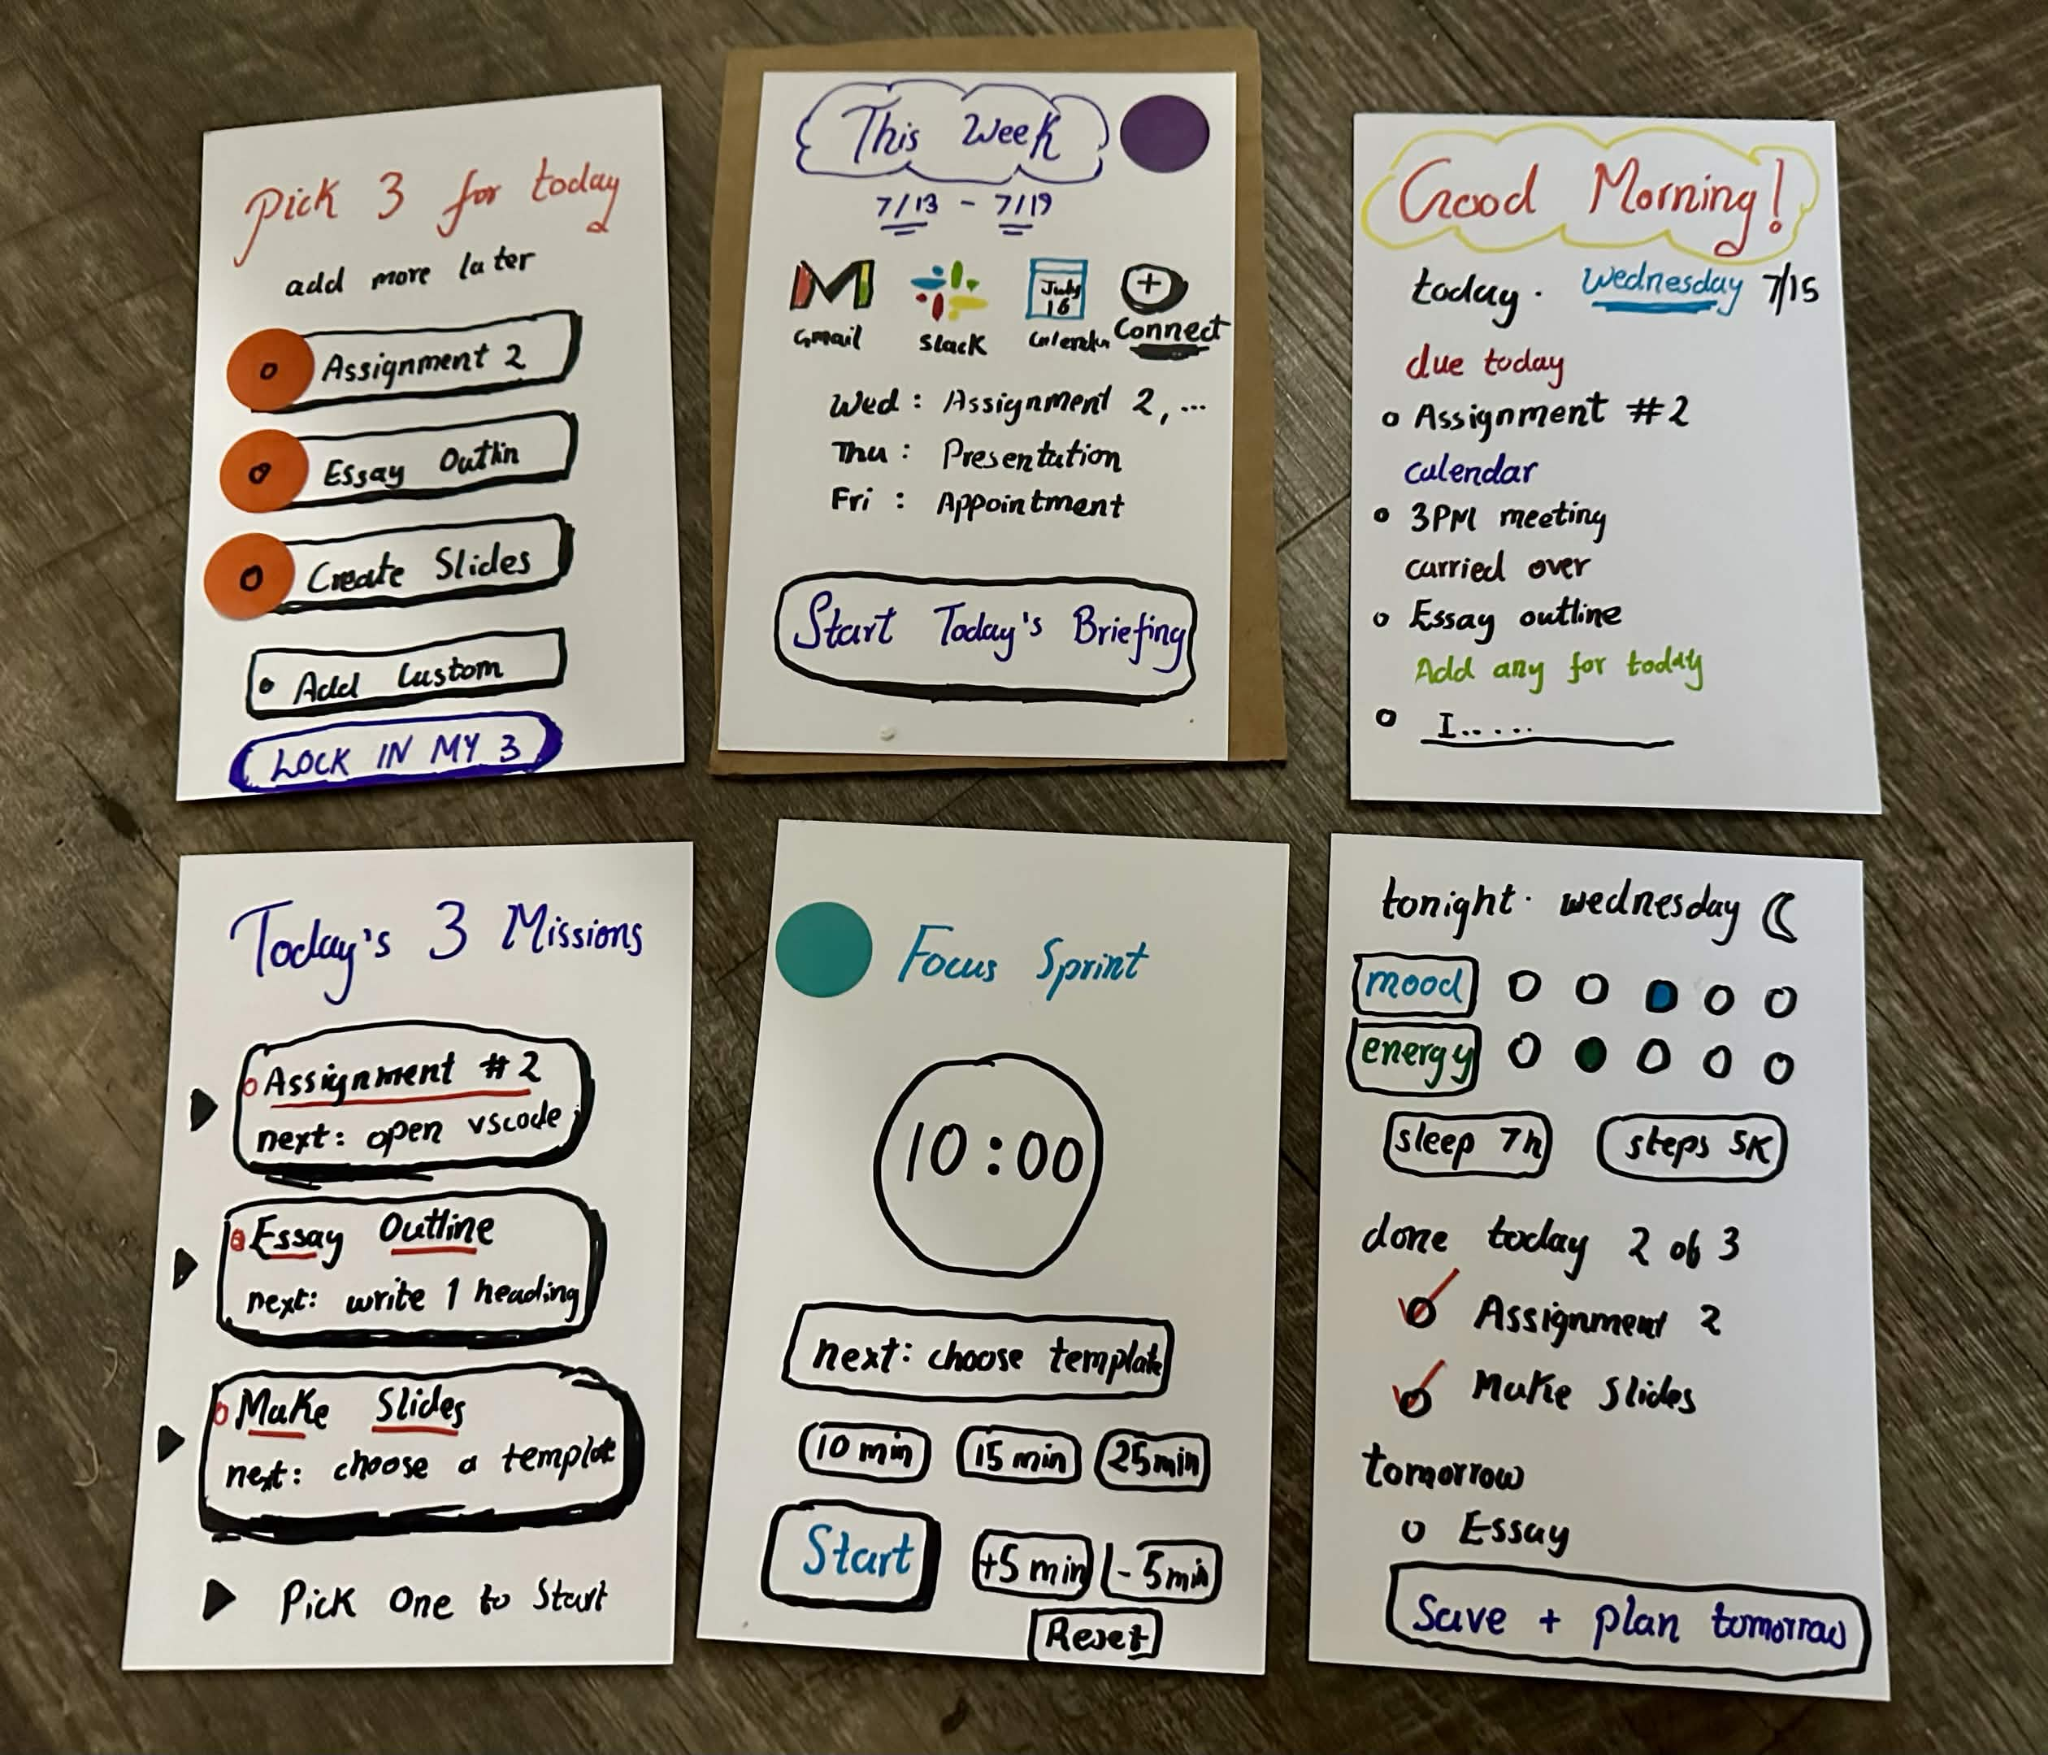
\includegraphics[width=\linewidth]{prototype-a-cards}
  \caption{Paper Prototype A: the six dashboard screens (This Week, Morning Briefing, Pick 3 for Today, Today's 3 Missions, Focus Sprint, and Night Reflection).}
  \Description{Six hand-drawn paper prototype cards laid out on a wooden table: Pick 3 for today, This Week, Good Morning briefing, Today's 3 Missions, Focus Sprint timer, and a night reflection card.}
  \label{fig:protoa}
\end{figure}

\textbf{Prototype B: Conversational co-pilot.} Voice companion, delivers briefings as a conversational chat thread with quick-reply chips and audio, so planning feels like just answering a few messages (Figure~\ref{fig:protob}). Navigation flow: a single scrolling chat thread with audio assistant, rather than a sequence of screens.

\begin{figure}[!ht]
  \centering
  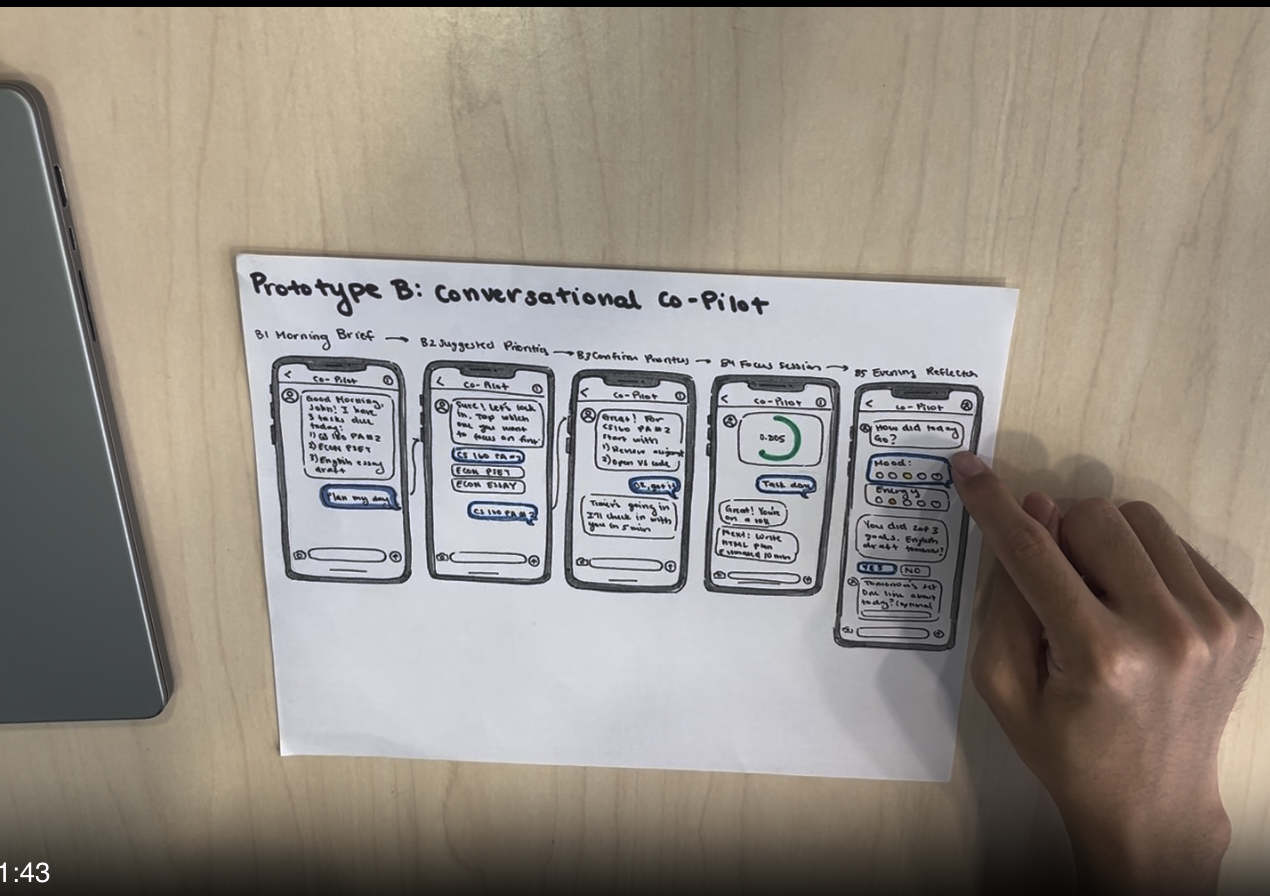
\includegraphics[width=\linewidth]{prototype-b-storyboard}
  \caption{Paper Prototype B: the conversational co-pilot storyboard, from morning brief through focus session to evening reflection.}
  \Description{Storyboard of five hand-drawn phone frames showing a chat-based co-pilot guiding the user from a morning brief to an evening reflection.}
  \label{fig:protob}
\end{figure}


\subsection{Findings}
We tested each prototype with three participants using a think-aloud protocol (Figures~\ref{fig:testa}--\ref{fig:testb}). Prototype A was praised more often than Prototype B. The core idea (consolidate scattered obligations, narrow to a next action) consistently landed, while the failure modes were about how much the app shows and asks.

\begin{figure}[!ht]
  \centering
  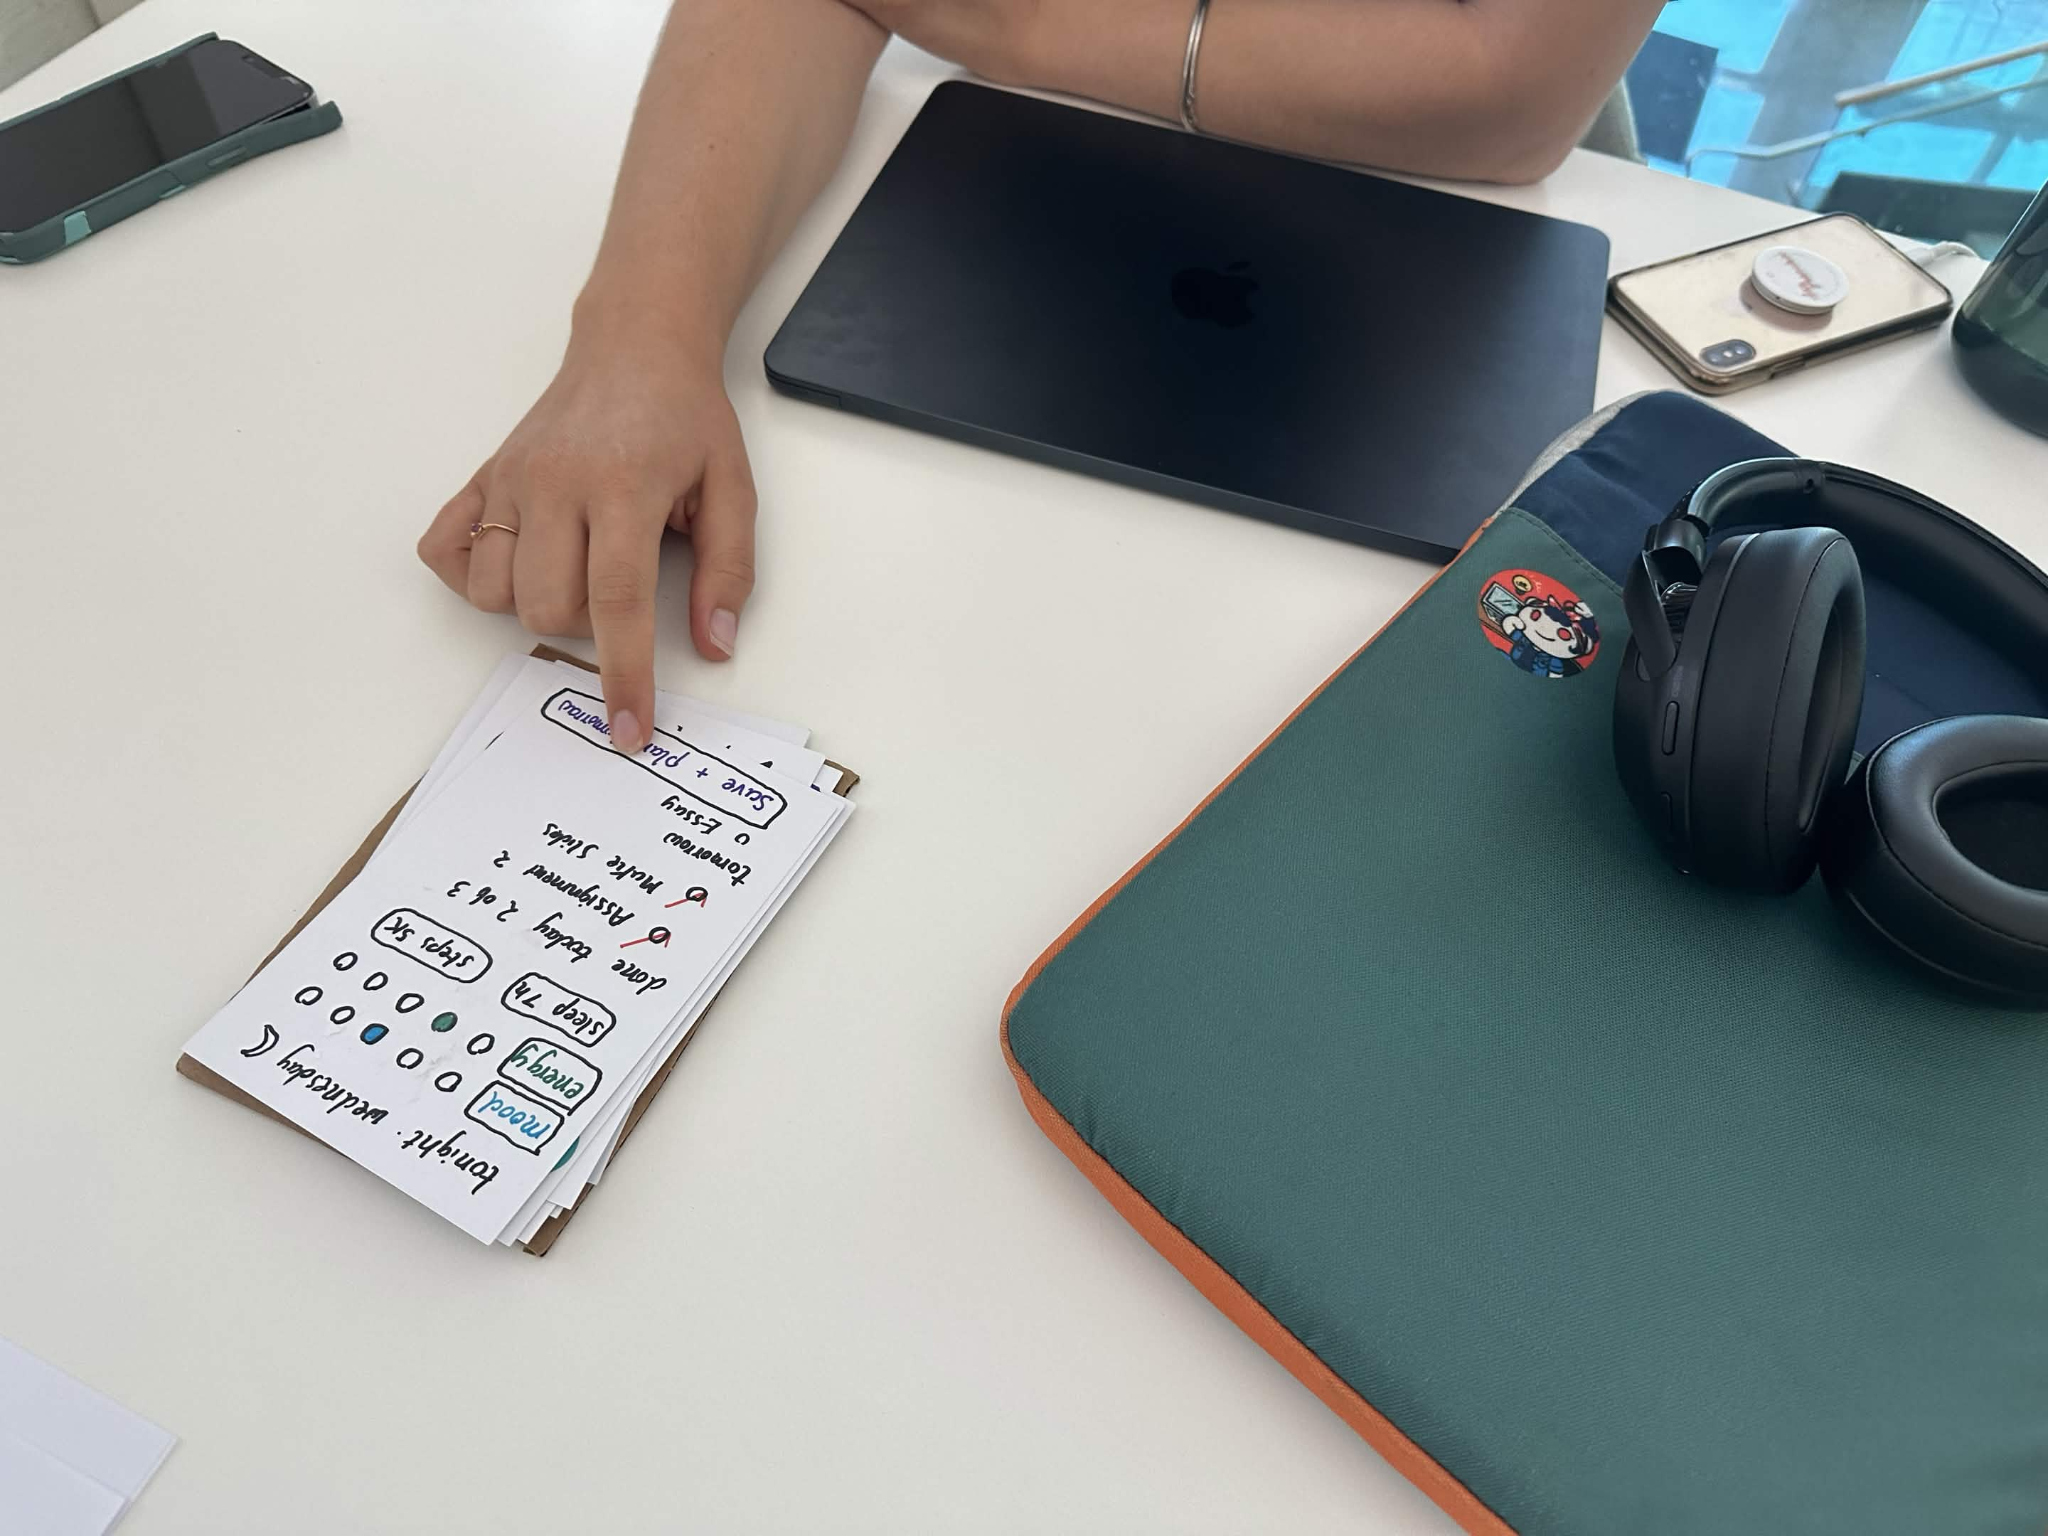
\includegraphics[height=1.5in]{testing-a-reflection}\hfill
  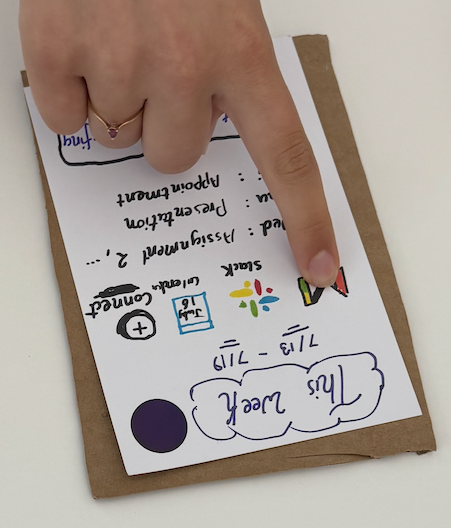
\includegraphics[height=1.5in]{testing-a-week}
  \caption{Think-aloud testing of Prototype A: reviewing the night reflection (left) and the This Week overview (right).}
  \Description{Two photos of participants pointing at paper prototype cards during think-aloud sessions.}
  \label{fig:testa}
\end{figure}


\begin{figure}[!ht]
  \centering
  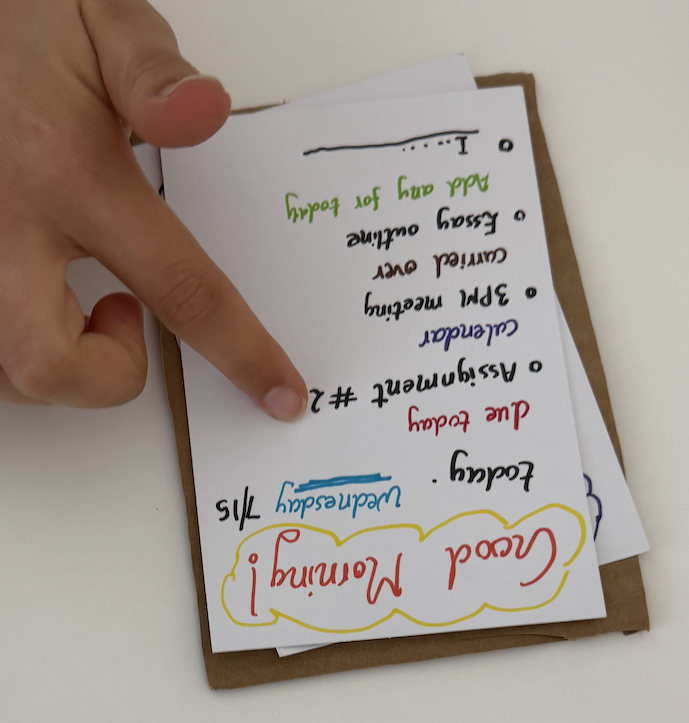
\includegraphics[width=.32\linewidth]{testing-a-briefing}\hfill
  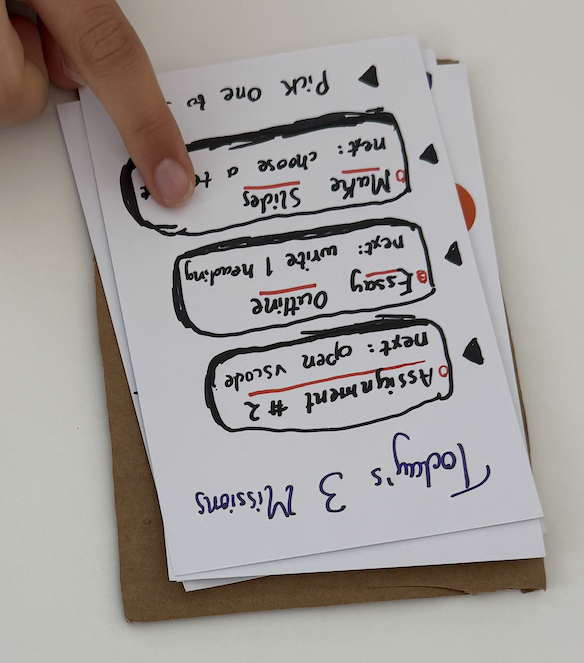
\includegraphics[width=.31\linewidth]{testing-a-missions}\hfill
  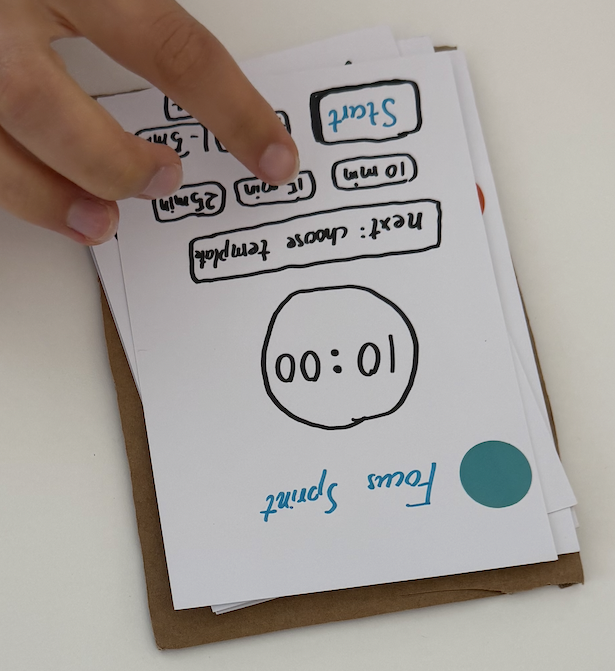
\includegraphics[width=.32\linewidth]{testing-a-sprint}
  \caption{Participants completing the three core tasks on Prototype A: morning briefing, Today's 3 Missions, and the Focus Sprint timer.}
  \Description{Three photos of participants tapping the Good Morning briefing card, the Today's 3 Missions card, and the Focus Sprint timer card.}
  \label{fig:testa2}
\end{figure}

\begin{figure}[!ht]
  \centering
  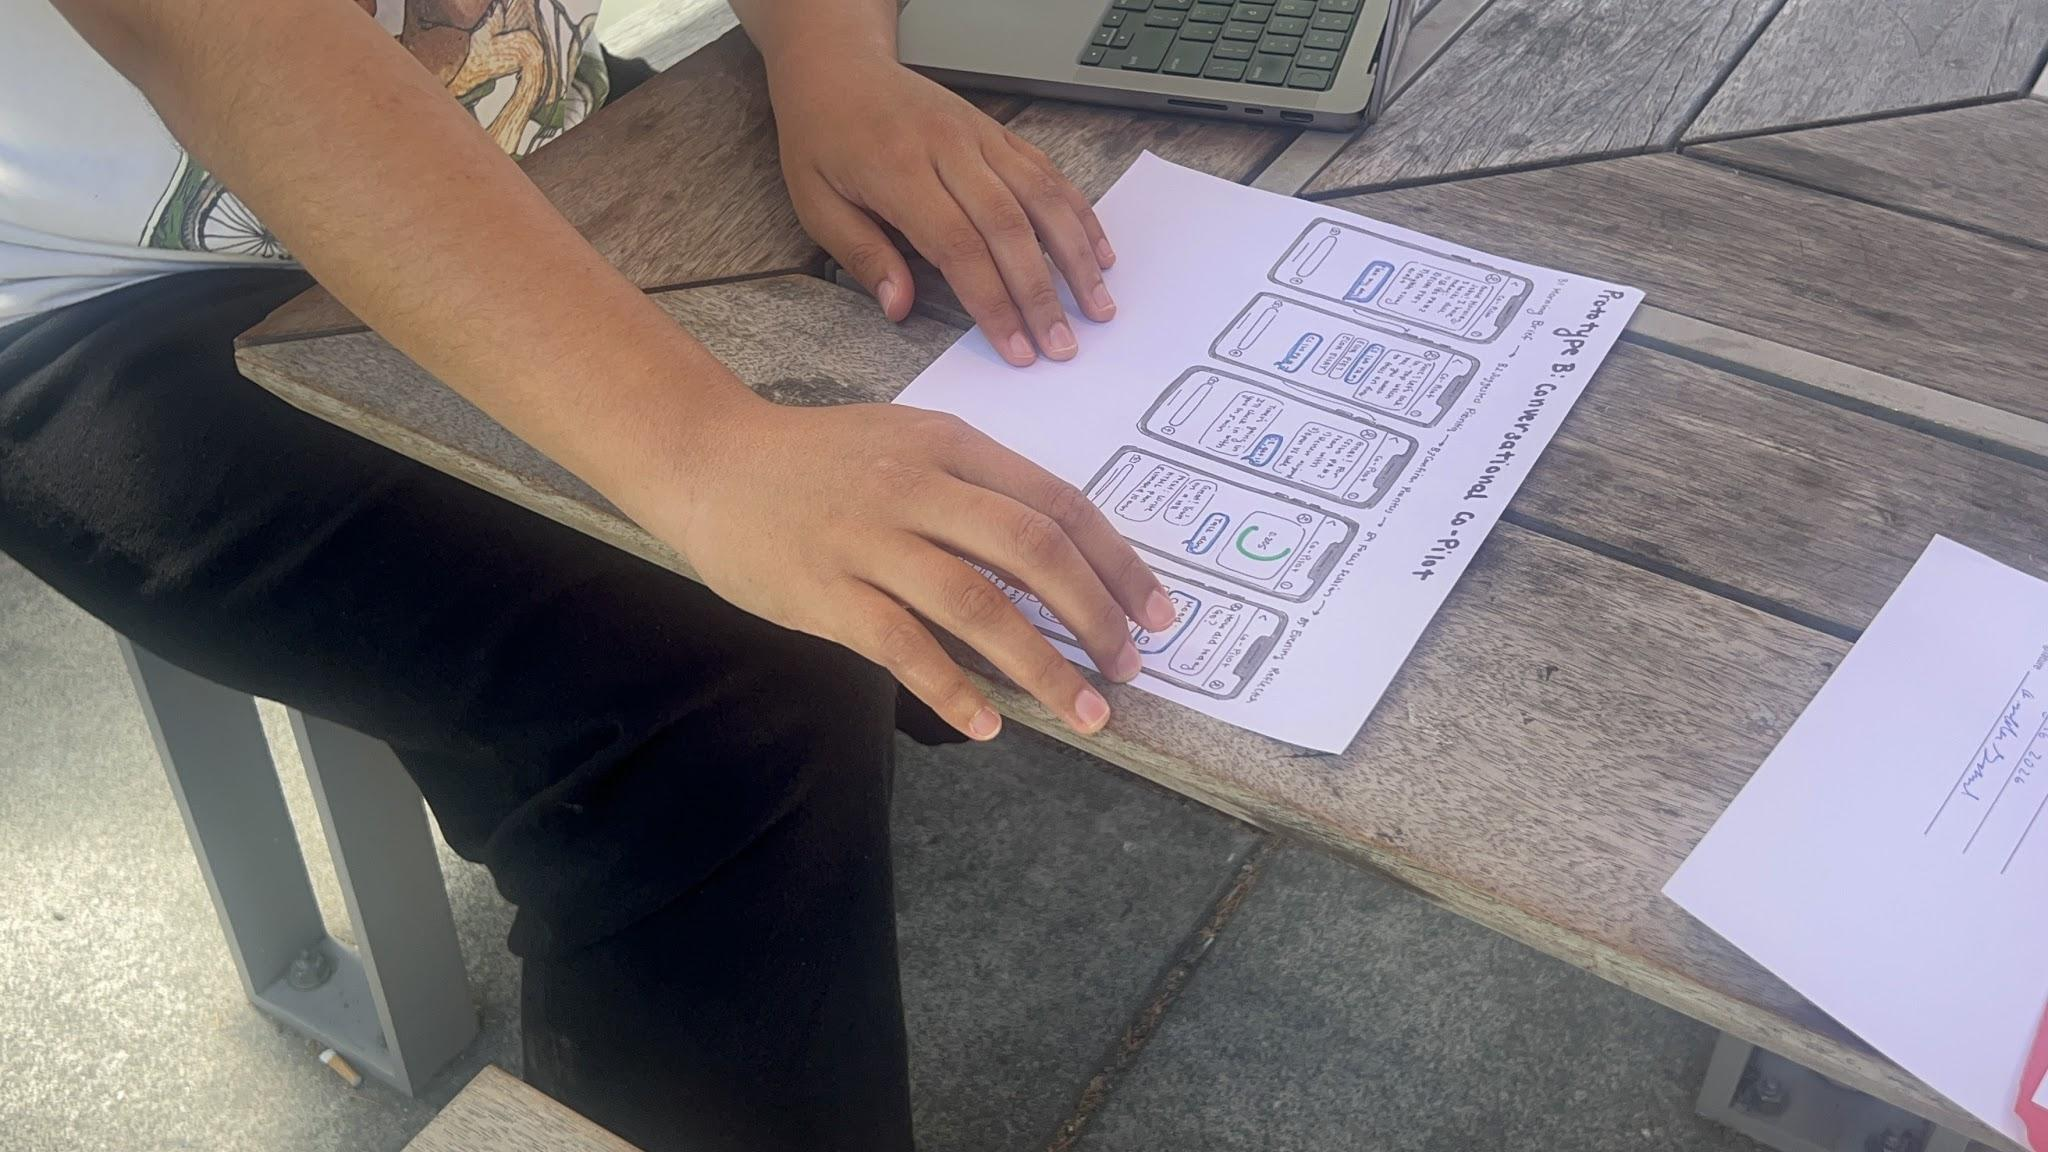
\includegraphics[height=1.4in]{testing-b-outdoor}\hfill
  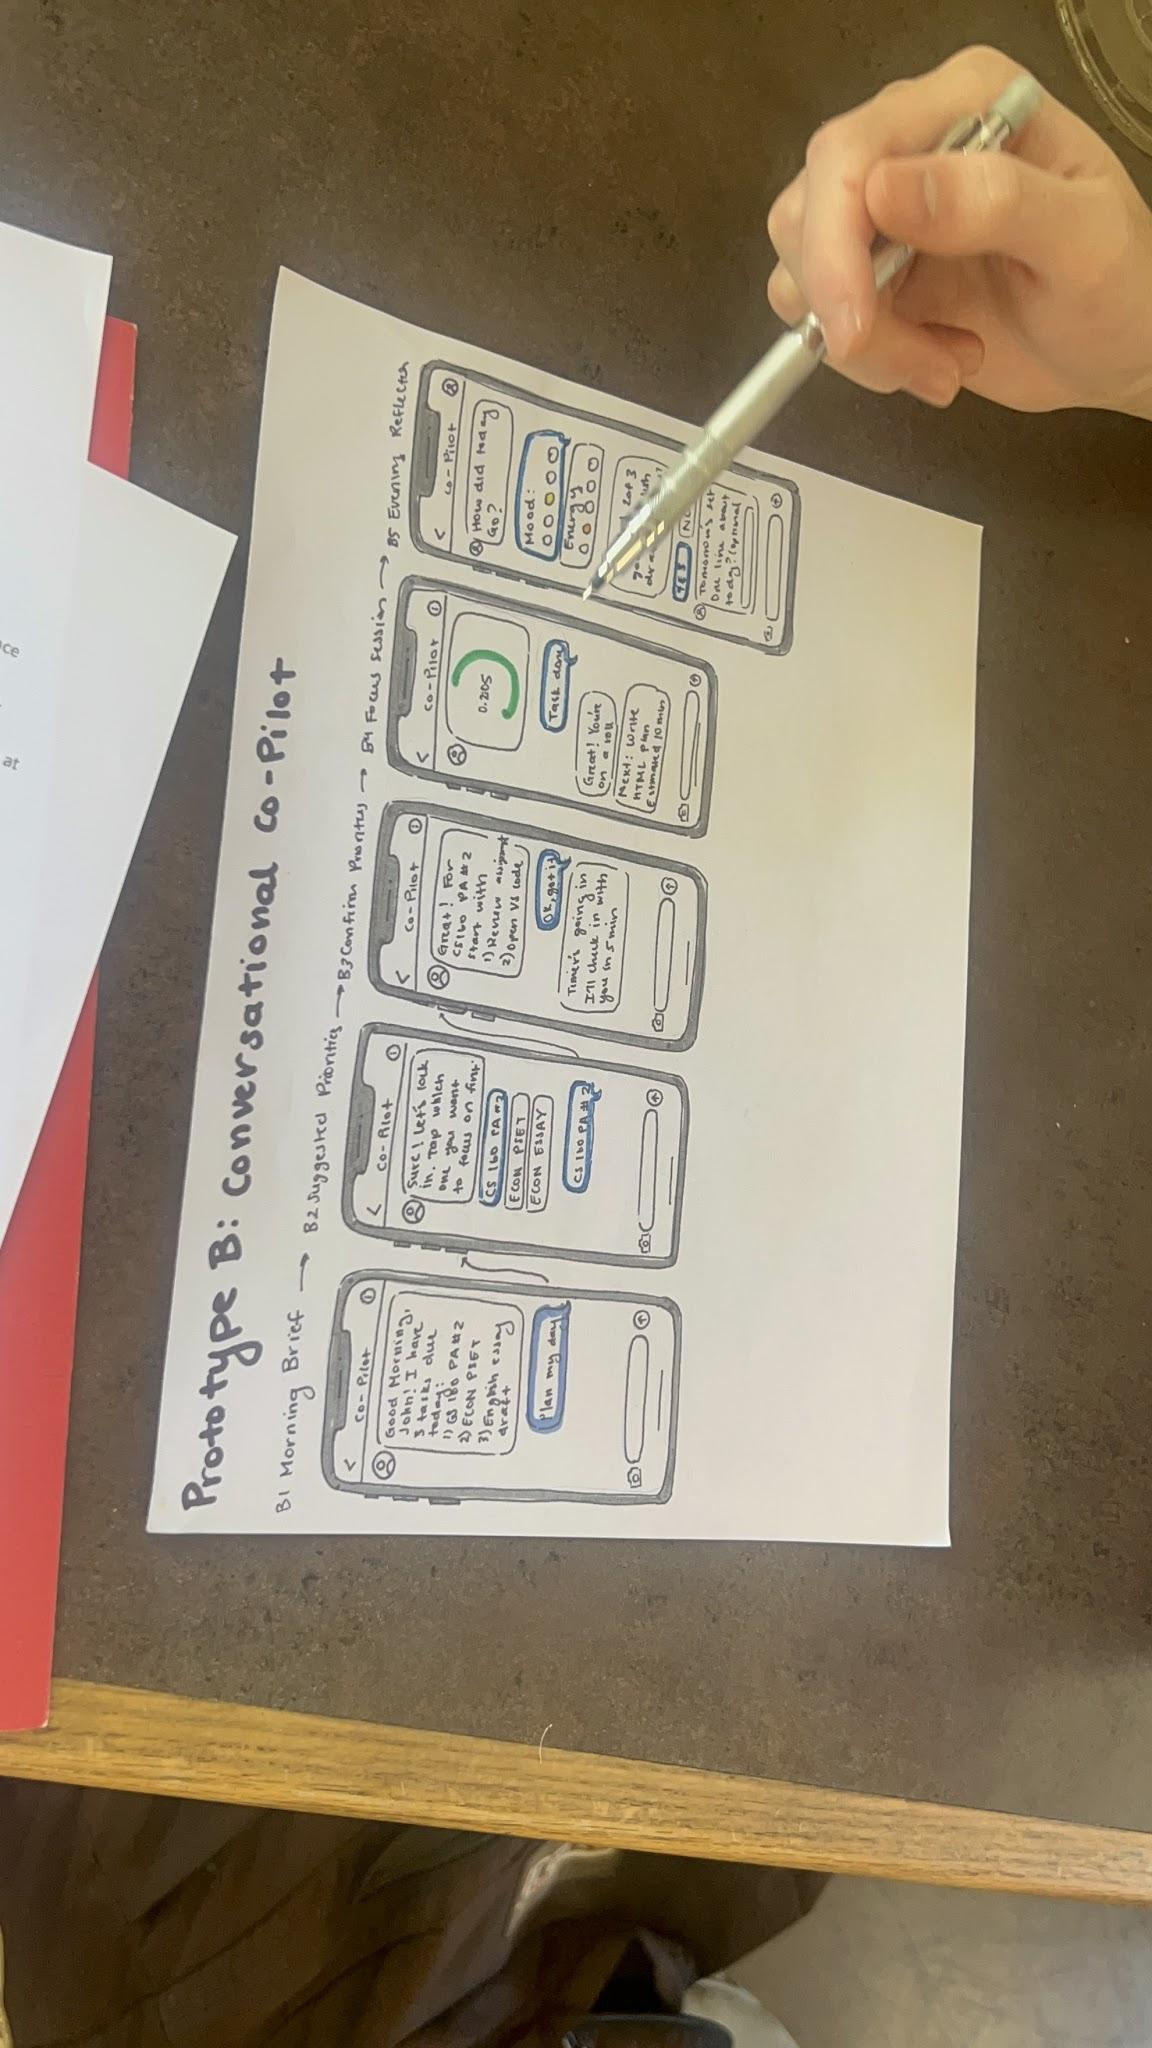
\includegraphics[height=1.4in]{testing-b-walkthrough}
  \caption{Prototype B think-aloud sessions.}
  \Description{Two photos of participants walking through the Prototype B storyboard, one outdoors at a wooden table and one pointing with a pen.}
  \label{fig:testb}
\end{figure} Common patterns across both prototypes are that users value simplicity and easy navigation while under the circumstances of dealing with tasks. Users value the idea of consolidation, only 3 tasks at one time, starting a focus session without overthinking, rollover tasks, one tiny step at a time, and the clear copilot chat flow.

We all agreed on adopting the concept of Prototype A; however, there are some common usability issues in Prototype A, such as an ambiguous starting point, unnecessary mood and energy tracking, missing due time, false affordances, and the burden of adjusting the task plan. Therefore, we planned changes for the next iteration: open on today's briefing by default, add a guided first run, make source icons functional buttons, make wellness tracking optional, differentiate the two selection screens, and attach times and pre-deadline alerts to tasks.

\section{Hi-Fi Prototyping}
Three team members independently designed high-fidelity single-screen mockups exploring different visual directions for the same core flow. Design 1 used a green-and-yellow palette with strong task-list organization but was critiqued for an unclear active-navigation state. Design 2 used a cohesive sage-green and neutral palette, explicitly built around a calming, wellness-oriented aesthetic, and most clearly supported breaking tasks into smaller steps. Design 3 offered a clean, minimal interface but was missing core features our concept depended on, including task breakdowns and focus sessions.

We selected Design 2, both for its alignment with our target users' need for a calm, non-overwhelming interface, and because its visual language could extend naturally to a ``Growth Garden'' progress visualization we had identified as a stretch goal.

%% To add a hi-fi screenshot later: drop the image in this folder and use
%% \includegraphics[width=.7\linewidth]{hifi-today} in a figure block here.

We then built a full interactive Figma prototype and tested it with six external participants. Three recurring themes emerged:
\begin{enumerate}
  \item Visual customization. Five of six participants wanted more visual customization, several explicitly describing the fixed green palette as a limiting factor in their willingness to adopt the app.
  \item Timer flexibility. Four of six participants wanted a more flexible focus timer, including custom durations rather than fixed five-minute increments, and a wider range of ambient sound options.
  \item Unclear text and interactions. Several participants found specific text and interactions unclear, including the meaning of ``Anchor 1 is next'' on the home screen, how rollover tasks worked, and a desire for clearer visual distinction between completed and incomplete tasks.
\end{enumerate}

In response, we planned a user-selectable accent color system, an adjustable timer, and a broader revision pass on the Today screen's copy and task states, all of which carried directly into implementation.

At this stage we also finalized our app's identity: the name Anchor, a minimal anchor-in-a-circle logo, and the tagline ``Steady the day,'' chosen to reflect the app's core philosophy of narrowing an overwhelming day down to a small, steady set of priorities.

\section{Implementation}
Anchor is implemented as a React 18 single-page application, built and bundled with Vite. Routing uses React Router in hash mode, which lets the app be hosted as a static site without server-side routing support, a necessary constraint given our deployment target of GitHub Pages via the gh-pages package.

For authentication and data persistence, we used Supabase, providing both a Postgres database and built-in authentication (email/password sign-up, password reset, and Google as a sign-in provider). We designed the data layer to be offline-first: a user's plan, reflections, and focus sessions are read from and written to localStorage immediately, with Supabase acting as a syncing layer that pulls and merges account data on sign-in. This meant the app remained fully usable without an account, and signing in later did not require migrating or losing local progress. Supabase's row-level security policies scope every read and write to the authenticated user's own ID, so no user's plan is visible to another.

Google Calendar and Gmail access uses the \texttt{@react-oauth/}\allowbreak\texttt{google} library, requesting read-only scopes and storing the resulting access token locally for use in subsequent API calls. Because the app has no backend server, this is a fully client-side OAuth flow using PKCE (Proof Key for Code Exchange) rather than the implicit flow, chosen specifically because implicit tokens are returned in the URL hash fragment, which would otherwise collide with React Router's own use of the hash for client-side routing. Gmail messages are filtered by a fixed query (unread, excluding Promotions and Social categories) before being surfaced as task candidates, a decision made after concluding that presenting a user's entire inbox as ``tasks'' would work against the app's goal of reducing, not adding to, daily cognitive load.

Styling follows a token-based CSS system derived directly from our Figma file, using CSS custom properties for color, spacing, and radius values so that a single accent-color change, offered to the user in Settings, propagates consistently across every screen, including a distinct dark mode.

Before evaluation, we ran a structured round of feature and stress testing across the full application, covering authentication, navigation, data persistence, the Morning Briefing, the focus timer, task rollover, Google integration, and manual task entry. This testing surfaced and resolved several real bugs, including anchors not saving to Today after briefing selection, timer audio continuing to play after the timer was paused, and postponed tasks not actually persisting to the next day. It also surfaced one open issue not yet fixed: calendar dates were generated in UTC while day-matching logic used local time, causing tasks to appear on the wrong day for users in timezones ahead of UTC. Stress testing (long input strings, corrupted local storage, rapid repeated input, large data volumes) found the app's existing validation and fallback handling to be robust in most cases, with the timezone bug as the one confirmed exception.

\section{User Evaluation}
We conducted a think-aloud evaluation with five participants, each completing the three primary tasks defined in Section 4: planning the day from scattered inputs, starting the next action, and closing out the day with rollover. Sessions were screen-recorded if the participant was comfortable, also recording audio of responses, otherwise we took notes; each ran 30 to 45 minutes, and participants completed a post-task Likert survey and an open-ended debrief.

Open-ended questions, asked conversationally:
\begin{itemize}
  \item Overall, how did that feel compared to how you currently keep track of your day?
  \item Was there any moment where you weren't sure what to do next? Walk me through what you were thinking there.
  \item What's one thing you'd want changed before you'd actually use this daily?
  \item Was there anything that surprised you in a good or bad way?
\end{itemize}

\begin{table*}
  \caption{Evaluation metrics, targets, and aggregate results across the five participants}
  \label{tab:metrics}
  \begin{tabular}{p{1.5in}p{2.7in}p{2.3in}}
    \toprule
    Metric & Target & Result\\
    \midrule
    Task completion & $\geq$80\% of participants complete each task independently & \\
    Time on task & Under 2 minutes & \\
    Taps/clicks to completion & Minimize unnecessary steps. Targeted: Task 1: 5, Task 2: 10, Task 3: 5 & \\
    Screens per task & Minimize unnecessary navigation.& \\
    Assists needed & No facilitator assistance for at least 4 of 6 participants per task & \\
    Errors / wrong turns & $\leq$1 error per task on average & \\
    \bottomrule
  \end{tabular}
\end{table*}

\subsection{Quantitative Results}
Table~\ref{tab:metrics} summarizes our pre-registered metrics and targets against the aggregate results; Figure~\ref{fig:survey} shows the post-task survey responses, and Figure~\ref{fig:quant} shows average time on task and first-attempt completion rates. Task 1 (Plan today) and Task 3 (Close out the day) were completed successfully, without facilitator intervention, by 4 of 5 participants. Task 2 (Start the next action) was the clear outlier: only 1 of 5 participants completed it without help, with the other four either failing on first attempt or requiring direct instruction.

\begin{figure}[!ht]
  \centering
  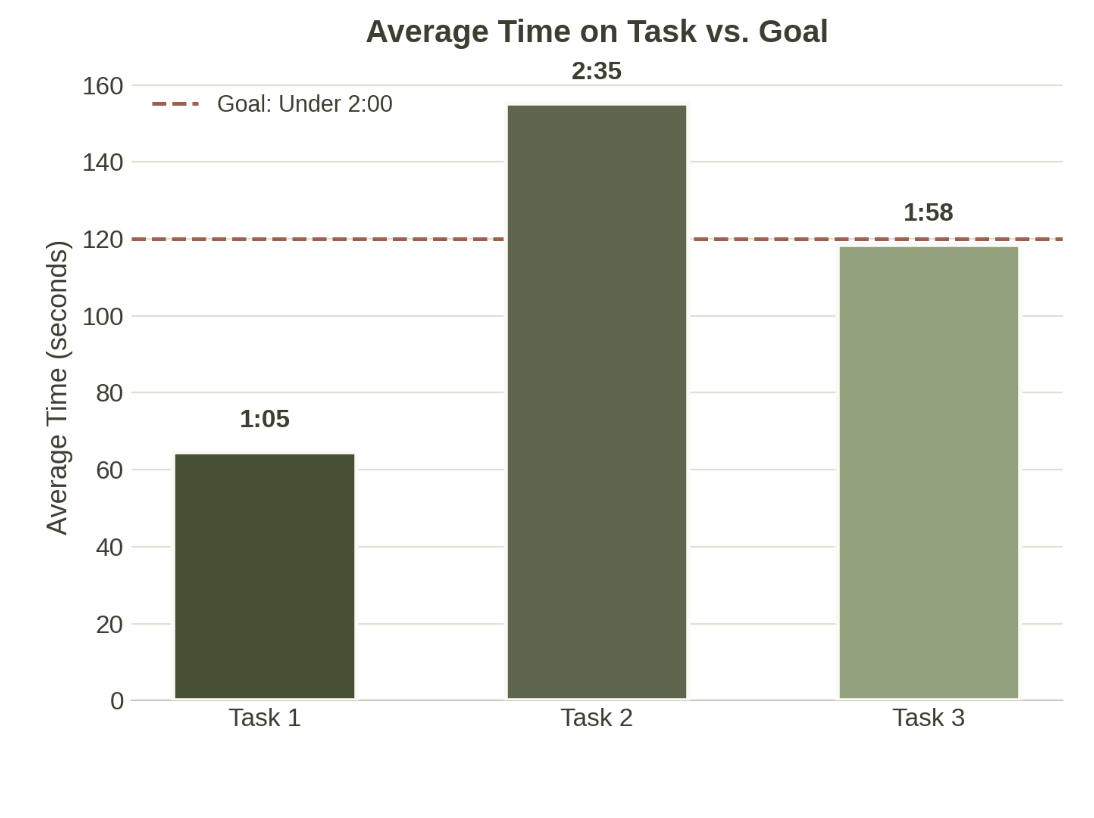
\includegraphics[width=.8\linewidth]{time-on-task}\\[4pt]
  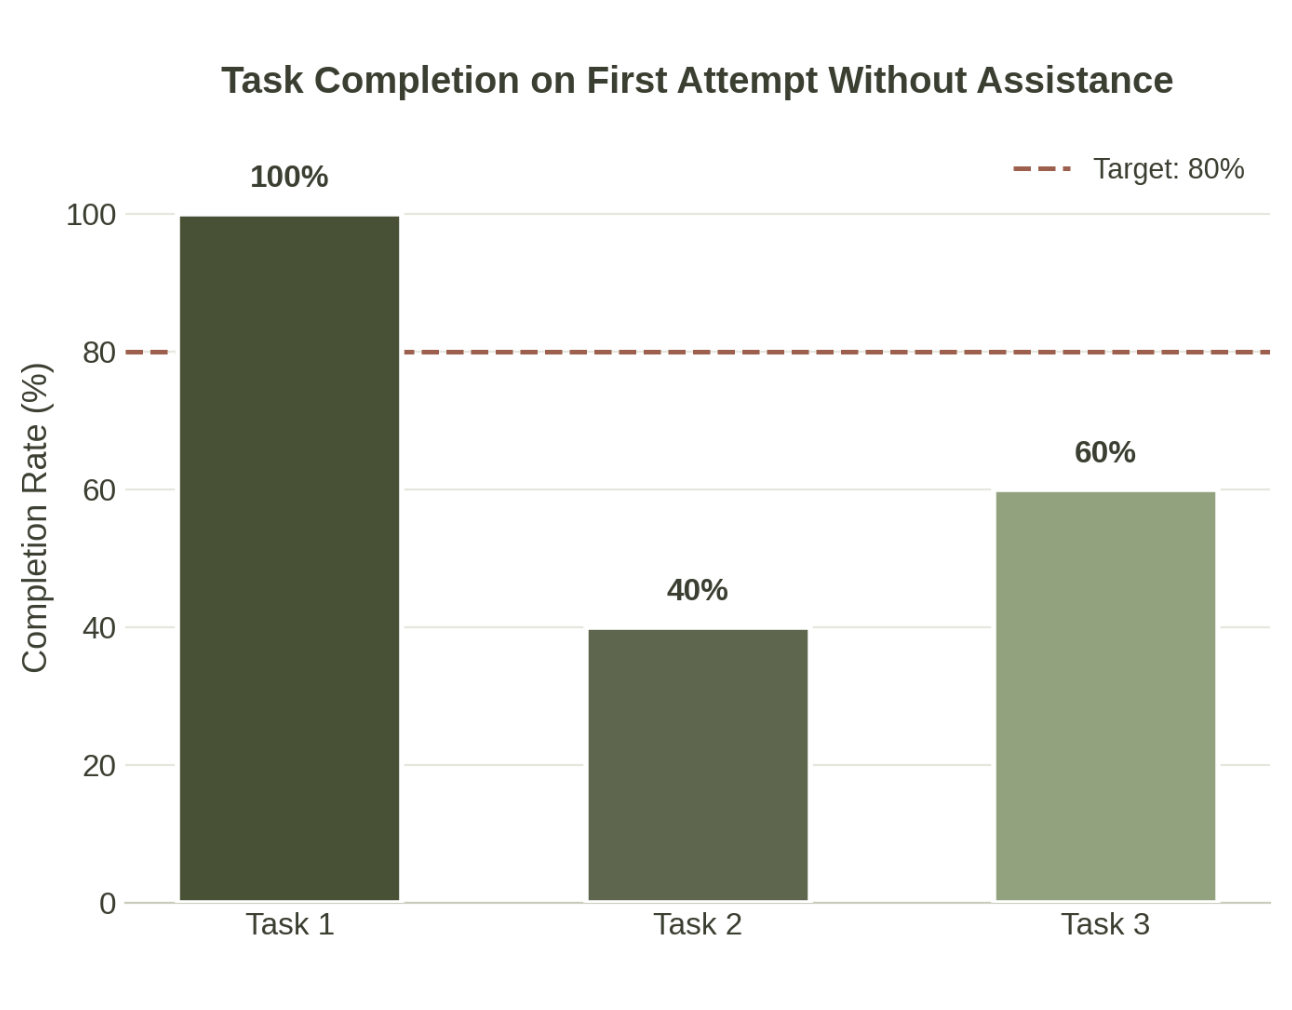
\includegraphics[width=.8\linewidth]{completion-rate}
  \caption{Average time on task versus the two-minute goal (top), and first-attempt completion without assistance versus the 80\% target (bottom). Task 2 (start the next action) missed both targets.}
  \Description{Two bar charts. Top: average times of 1:05, 2:35, and 1:58 for Tasks 1 to 3 against a dashed two-minute goal line. Bottom: completion rates of 100, 40, and 60 percent against a dashed 80 percent target line.}
  \label{fig:quant}
\end{figure}

Time on task followed the same pattern. Task 1 averaged just under a minute; Task 3 averaged under two minutes for most participants. Task 2 took substantially longer across the board, ranging from 1:26 up to 5:00, well past our 2-minute target for every participant except one.

Tap counts were similarly uneven. While several participants completed Task 1 near or under our target of 5 taps, Task 2 and Task 3 saw wide variance, including one participant needing 30 and 35 taps respectively for Task 2 and Task 3, far above target. Assist counts and error counts were highest on Task 2 and Task 3, with one participant needing 4 assists and encountering 6 errors on Task 1 alone.

Taken together, the quantitative data points to the same conclusion the qualitative coding independently reached: Task 2, starting a focus session, is where the app currently loses users.

\begin{figure*}
  \centering
  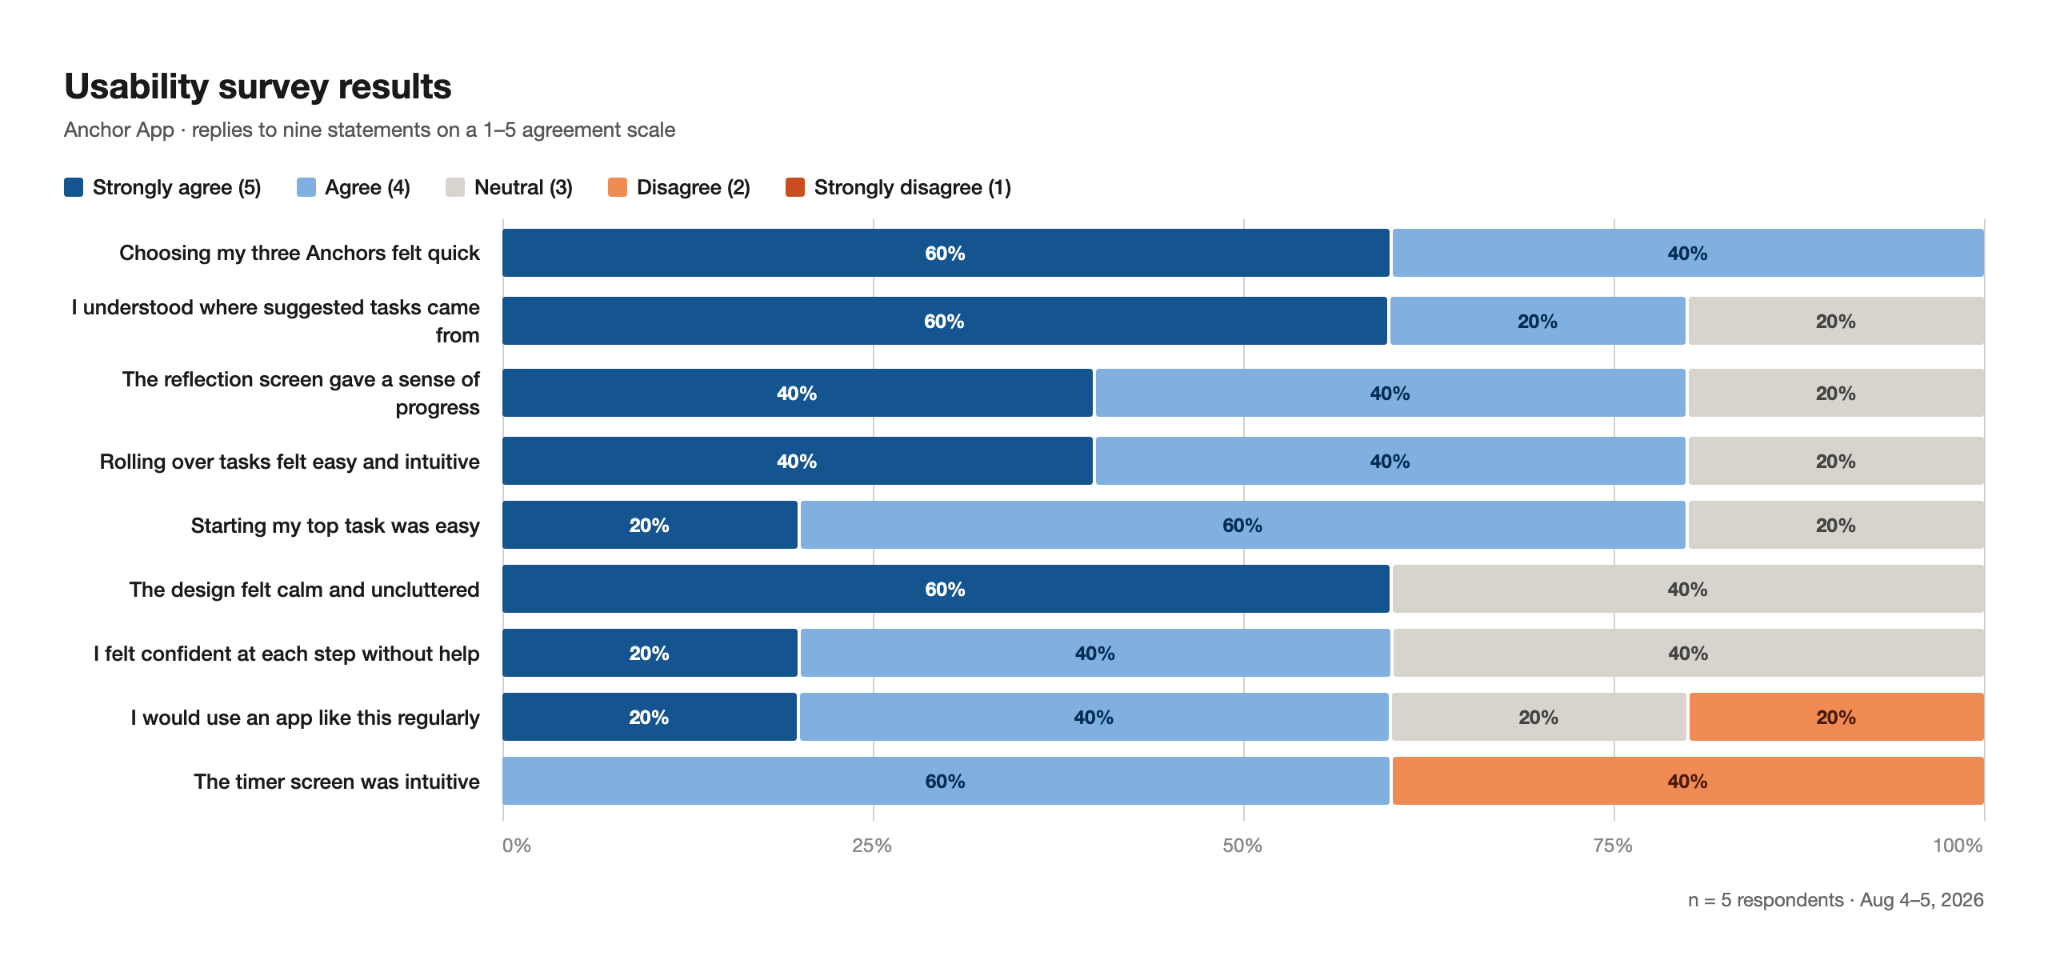
\includegraphics[width=.95\textwidth]{survey-results}
  \caption{Post-task usability survey results: nine statements on a 1--5 agreement scale (n = 5).}
  \Description{Stacked bar chart of survey responses. Choosing three anchors felt quick and the design felt calm scored highest; the timer screen was intuitive scored lowest, with 40 percent disagreement.}
  \label{fig:survey}
\end{figure*}

\subsection{Qualitative Findings}
We coded think-aloud transcripts and observation notes from all five sessions into 13 descriptive codes, which we grouped into three usability themes.

\textbf{Theme 1: Anchor's labels describe the app's own concepts rather than the action they perform.} Three participants stalled on at least one label. One participant did not recognize “choose an anchor” as meaning “choose a task” and directly suggested simpler wording. Another asked, “What’s today’s anchors section?” and separately did not recognize “Start weekly briefing” as an actionable button. The “Start 5 min” label was the most consistent point of confusion, with participants unable to tell whether it meant the task would take five minutes or whether it would start a five-minute timer.

\textbf{Theme 2: The app gives little feedback about what an action did, and offers few ways to undo or exit.} One participant finished a focus session early but found no way to end it or leave the timer screen; the timer overlay also blocked navigation while she was stuck. The same participant tried to reverse an “I started” state after tapping it, but did not receive a response. Three participants separately looked for an end-of-session sound or vibration that did not exist. Several participants also wanted visible due dates and clearer date labeling, information the app currently does not surface.

\textbf{Theme 3: The features participants valued most were consistently the ones they discovered last.} Three participants gave unprompted praise to the Garden screen once they found it, with one comparing it favorably to her current calendar-and-reminders workflow. However, Garden was not part of the core task flow and had to be discovered independently. One participant never navigated to Reflection without prompting and later described it as unclear it functioned as the day’s closing step. Multiple participants explicitly said the app made more sense on a second pass than on the first.

\subsection{Next Steps}
Based on these findings, we identified five concrete changes for our next iteration:
\begin{enumerate}
  \item Add a first-run guided walkthrough that runs the full loop once with sample content, since every participant needed a second pass before the app's structure made sense.
  \item Rename product-specific labels to familiar action words, replacing ``Anchor'' and ``Start 5 min'' with plainer language like ``task'' and clearer action framing, while keeping ``Anchor'' as the app's name rather than its interface vocabulary.
  \item Make every action reversible and confirmed, including an exit and ``done'' control on the timer, an editable ``I started'' state, and confirmation messages with undo for destructive actions like clearing tasks.
  \item Add optional notifications, sound, and vibration for the end of the session and upcoming due times, addressing the repeated request for an audible or physical signal rather than requiring users to check the screen.
  \item Surface due dates and deadlines directly on tasks, and roll missed, unscheduled deadlines forward automatically rather than letting them silently disappear.
\end{enumerate}

\section{Conclusion}
Anchor began with a specific, recurring observation from our needfinding interviews: our participants’ struggle was rarely a lack of information or planning ability, but rather the absence of a small, bounded entry point into work they already understood. Every stage of our process—from choosing the unified-briefing concept over distraction blocking or social accountability, to removing mood and energy tracking after lo-fi testing, to adding user-selectable color themes after hi-fi critique—was driven by returning to that same core problem rather than adding features for their own sake.

Our final evaluation confirmed both the strengths and current limitations of this approach, since participants consistently valued a bounded plan, a reflection that reframes setbacks as information, and a visual sense of progress over time. However, the evaluation also showed that these benefits were often hidden behind unfamiliar language and unclear feedback, particularly at the exact moment—starting a task—that our needfinding identified as the most difficult for this user group.

Building the working application also revealed challenges that were difficult to anticipate during the design process. Implementing the app as a fully client-side, statically hosted application required us to work through constraints around OAuth authentication, offline-first data persistence, and coordinating contributions across a shared codebase.

We see Anchor not as a finished product but as a working demonstration that a genuinely small, honest daily plan can be more useful to an overwhelmed user than a more complete, more powerful system, provided that plan is also clear enough to trust on the first try.

\begin{acks}
Thank you so much to Selaine Rodriguez, Mina Huh, and our Teaching Assistant Vivian Shen for your guidance and feedback throughout the semester! Thank you to our classmates for their thoughtful feedback on our prototypes and for sharing your work with us. And a huge thank you to all of our interviewees, including friends who volunteered their time and Berkeley students we recruited on the spot, for sharing your experiences that helped shape our project.
\end{acks}

%% ------------------------------------------------------------------
%% Citations (optional). To cite related work:
%% 1. Add entries to a .bib file (e.g. anchor.bib in this folder).
%% 2. Uncomment the two lines below.
%% 3. Cite in text with \cite{key}.
%%
%% \bibliographystyle{ACM-Reference-Format}
%% \bibliography{anchor}
%% ------------------------------------------------------------------

\end{document}
